\chapter{DAKOTA Tutorial}\label{tutorial}

\section{Installation Guide}\label{tutorial:installation}

DAKOTA can be compiled for most common computer systems that run Unix
and Linux operating systems. The computers and operating systems
actively supported by the DAKOTA project include:

\begin{itemize}
\item Intel/AMD Redhat Enterprise Linux 4 and 5 (RHEL4, RHEL5) with gcc and Intel compilers
\item Sun Solaris 5.10 with SunPro CC compilers
\item IBM AIX 5.3 with xlC compilers
\item Mac OS X 10.5 with gcc compilers
\end{itemize}

In addition, partial support is provided for PC Windows (via Cygwin)
with gcc/g95 compilers, PC Windows (via MinGW) with gcc-4 compilers,
and Sandia's ASC Red Storm with PGI compilers. Additional details are
provided in the file \texttt{Dakota/README} in the distribution (see
the following section for download instructions).  Further
platform/operating system-specific guidance can be found in
Dakota/examples/platforms included with DAKOTA.

For answers to common questions and solutions to common problems in
downloading, building, installing, or running DAKOTA, refer to
\url{http://dakota.sandia.gov/faq.html} for additional information.

\subsection{How to Obtain DAKOTA - External to Sandia Labs}\label{tutorial:installation:how1}

Users outside of Sandia National Laboratories may obtain the DAKOTA
binary executable files and source code files through the download
link available here:\smallskip

\url{http://dakota.sandia.gov/download.html}

To receive the binary or source code files, you are asked to fill out
a short online registration form. The information provided is used by
the DAKOTA development team to collect software usage metrics; the
form also lets you sign up for update announcements.

If you wish to run DAKOTA on one of the supported or partially
supported platforms, we suggest that you download the relevant binary
executable distribution rather than the source code distribution. This
gets you up and running quickly and lets you gain an understanding of
DAKOTA by running the example problems that are provided with the
binary distributions.  For more experienced users, DAKOTA can be
customized with additional packages and ported to other computer
platforms when building from the source code.

\subsection{How to Obtain DAKOTA - Internal to Sandia Labs}\label{tutorial:installation:how2}

DAKOTA binary executable files are routinely compiled and distributed
to the engineering sciences LANs and common compute servers at Sandia,
Los Alamos, and Lawrence Livermore.  At Sandia, consult the
Codes \& Tools tab of the computing.sandia.gov web portal
% analyst home page
or the DAKOTA internal webpage for specific installation
locations and preferred usage.  These installations are typically
supported by modules, e.g., \texttt{module avail dakota}.  However,
binaries can be located by absolute path as well, e.g.,
\texttt{/usr/local/dakota/bin/dakota} or
\texttt{/projects/dakota/bin/<system>/dakota}, where
``\texttt{<system>}'' is \texttt{linux64}, \texttt{osx}, or other.  To
see if DAKOTA is available on your computer system and accessible in
your Unix environment path settings, type the command \texttt{which
dakota} at the Unix prompt. If the DAKOTA executable file is in your
path, its location will be echoed to the terminal. If the DAKOTA
executable file is available on your system but not in your path, then
you will need to locate it and add its directory to your path (the
Unix \texttt{whereis} and \texttt{find} commands can be useful for
locating the executable).

If DAKOTA is not available on your system, consider getting an account
on one of the common compute servers where DAKOTA is maintained.  If
not practical, visit the DAKOTA internal webpage or consult the DAKOTA
developers so we can provide you with the most complete DAKOTA
distribution possible, i.e., including Sandia-specific and/or
site-licensed software.  As a last resort, you can acquire external
versions of DAKOTA as described above.

\subsection{Installing DAKOTA - Binary Executable Files}\label{tutorial:installation:installing1}

Once you have downloaded a binary distribution from the web site
listed above, you will have a Unix tar file that has a name similar to
\texttt{Dakota\_5\_x.OSversion.tar.gz}.

Use the GNU utility \texttt{gunzip} to uncompress the tar file and
the Unix \texttt{tar} utility to extract the files from the archive by
executing the following commands:
\begin{small}
\begin{verbatim}
    gunzip Dakota_5_x.OSversion.tar.gz
    tar -xvf Dakota_5_x.OSversion.tar
\end{verbatim}
\end{small}
Slightly faster and less demanding of disk space is to invoke
\begin{small}
\begin{verbatim}
    gzip -dc Dakota_5_x.OSversion.tar.gz | tar xf -
\end{verbatim}
\end{small}

The tar utility will create a subdirectory named \texttt{Dakota} in
which the DAKOTA executables and example files will be stored. The
executables are in \texttt{Dakota/bin}, and the example problems are
\texttt{Dakota/test} and in subdirectories of \texttt{Dakota/examples}.
See file \texttt{Dakota/examples/README} for more details about these
subdirectories.

A similar process applies to windows distributions which are packaged
as ZIP files and can be extracted with the Windows extractor or
WinZIP, for example.  For getting started on Windows, see the
files \texttt{INSTALL.cygwin} and \texttt{INSTALL.mingw} in
\texttt{Dakota/examples/platforms}.

\subsection{Installing DAKOTA - Source Code Files}\label{tutorial:installation:installing2}

Following the download, decompression, and extraction of the file
\texttt{Dakota\_5\_x.src.tar.gz}, the basic steps follow the standard
GNU distribution process of:
\begin{small}
\begin{verbatim}
    configure
    make
\end{verbatim}
\end{small}
to construct Makefiles and build the system, respectively.  After the build
complete, one can optionally
\begin{small}
\begin{verbatim}
    make install
\end{verbatim}
\end{small}
to install the executable in a desired location.  Please note that these
simple steps imply a build process in which the configuration, object files,
libraries, and binary executables all reside in the same directory as the
extracted Dakota source distribution.  Many developers on the DAKOTA
development team use this approach so it is encouraged.  That said, DAKOTA
does support out-of-source build trees as long as GNU make (or other make
installation that supports VPATH variable) is used.  Detailed instructions
for building DAKOTA are given in the file
\texttt{Dakota/INSTALL}.

\subsection{Running DAKOTA}\label{tutorial:installation:running}

The DAKOTA executable file is named dakota. If this command is entered
at the command prompt without any arguments, the following usage message
appears (please ensure '.' is in your PATH):
\begin{small}
\begin{verbatim}
usage: dakota [options and <args>]
        -help (Print this summary)
        -version (Print DAKOTA version number)
        -input <$val> (REQUIRED DAKOTA input file $val)
        -output <$val> (Redirect DAKOTA standard output to file $val)
        -error <$val> (Redirect DAKOTA standard error to file $val)
        -parser <$val> (Parsing technology: nidr[strict][:dumpfile])
        -check (Perform input checks)
        -pre_run [$val] (Perform pre-run (variables generation) phase)
        -run [$val] (Perform run (model evaluation) phase)
        -post_run [$val] (Perform post-run (final results) phase)
        -read_restart [$val] (Read an existing DAKOTA restart file $val)
        -stop_restart <$val> (Stop restart file processing at evaluation $val)
        -write_restart [$val] (Write a new DAKOTA restart file $val)
\end{verbatim}
\end{small}
%$ this comment is here to trick xemacs into highlighting syntax correctly

Of these available command line inputs, only the ``\texttt{-input}''
option is required, and ``\texttt{-input}'' can be omitted if the
input file name is the final item on the command line; all other
command-line inputs are optional. The ``\texttt{-help}'' option prints
the usage message above. The ``\texttt{-version}'' option prints the
version number of the executable. The ``\texttt{-check}'' option
invokes a dry-run mode in which the input file is processed and
checked for errors, but the study is not performed. The
``\texttt{-input}'' option provides the name of the DAKOTA input file.
The ``\texttt{-output}'' and ``\texttt{-error}'' options provide file
names for redirection of the DAKOTA standard output (stdout) and
standard error (stderr), respectively.  The ``\texttt{-parser}'' input
is for debugging and will not be further described here.  The
``\texttt{-read\_restart}'' and ``\texttt{-write\_restart}'' command
line inputs provide the names of restart databases to read from and
write to, respectively. The ``\texttt{-stop\_restart}'' command line
input limits the number of function evaluations read from the restart
database (the default is all the evaluations) for those cases in which
some evaluations were erroneous or corrupted. Restart management is an
important technique for retaining data from expensive engineering
applications. This advanced topic is discussed in detail in
Chapter~\ref{usage}. Note that these command line inputs can be
abbreviated so long as the abbreviation is unique, so the following
are valid, unambiguous specifications: ``\texttt{-h}'',
``\texttt{-v}'', ``\texttt{-c}'', ``\texttt{-i}'', ``\texttt{-o}'',
``\texttt{-e}'', ``\texttt{-re}'', ``\texttt{-s}'', ``\texttt{-w}'',
``\texttt{-pr}'', ``\texttt{-ru}'', and ``\texttt{-po}'' and can be
used in place of the longer forms of the command line inputs.

To run DAKOTA with a particular input file, the following syntax can
be used:
\begin{small}
\begin{verbatim}
    dakota -i dakota.in
\end{verbatim}
\end{small}
or more simply
\begin{small}
\begin{verbatim}
    dakota dakota.in
\end{verbatim}
\end{small}

This will echo the standard output (stdout) and standard error
(stderr) messages to the terminal. To redirect stdout and stderr to
separate files, the \texttt{-o} and \texttt{-e} command line options
may be used:
\begin{small}
\begin{verbatim}
    dakota -i dakota.in -o dakota.out -e dakota.err
\end{verbatim}
\end{small}
or
\begin{small}
\begin{verbatim}
    dakota -o dakota.out -e dakota.err dakota.in
\end{verbatim}
\end{small}

Alternatively, any of a variety of Unix redirection variants can be
used. The simplest of these redirects stdout to another file:
\begin{small}
\begin{verbatim}
    dakota dakota.in > dakota.out
\end{verbatim}
\end{small}

To append to a file rather than overwrite it, ``\texttt{>>}'' is used
in place of ``\texttt{>}''. The syntax to redirect stderr as well as stdout
to the same file depends on the shell you are using.  With csh, simply append
``\texttt{\&}'' with no embedded space, i.e.,
``\texttt{>\&}'' or ``\texttt{>>\&}''. With the Bourne shell (sh or bash) use
``\texttt{>dakota.out 2>\&1}'' or ``\texttt{>>dakota.out 2>\&1}''.
With csh, if you have the noclobber environment variable set but
wish either to overwrite an existing output file or to append to a file that
does not yet exist, append ``\texttt{!}'' to the redirection operators
(with no intervening spaces), i.e.,
``\texttt{>!}'', ``\texttt{>\&!}'', ``\texttt{>>!}'', or
``\texttt{>>\&!}''.

To run the dakota process in the background, append an ampersand
symbol (\&) to the command with an embedded space, e.g.,
\begin{small}
\begin{verbatim}
    dakota dakota.in > dakota.out &
\end{verbatim}
\end{small}

Refer to~\cite{And86} for more information on Unix redirection and
background commands.

The ``\texttt{-pre\_run}'', ``\texttt{-run}'', and
``\texttt{-post\_run}'' switches instruct DAKOTA to run one or more
execution phases, excluding others.  For example pre-run might
generate variable sets, run (core run) invoke the simulation to
evaluate variables, producing responses, and post-run accepts
variable/response sets and analyzes the results (for example,
calculate correlations from a set of samples).  Currently only two
modes are supported and only for sampling, parameter study, and DACE
methods: (1) pre-run only with optional tabular output of variables:
\begin{small}
\begin{verbatim}
    dakota -i dakota.in -pre_run [::myvariables.dat]
\end{verbatim}
\end{small}
and (2) post-run only with required tabular input of variables/responses:
\begin{small}
\begin{verbatim}
    dakota -i dakota.in -post_run myvarsresponses.dat::
\end{verbatim}
\end{small}

 
\section{Rosenbrock and Textbook Test Problems}\label{tutorial:rosenbrock}

Many of the example problems in this chapter use the Rosenbrock
function \cite{Rosenbrock60} (also described in \cite{Gil81}, among
other places), which has the form:

\begin{equation}
f(x_1,x_2)=100(x_2-x_1^2)^2+(1-x_1)^2 \label{tutorial:rosen}
\end{equation}

A three-dimensional plot of this function is shown in
Figure~\ref{tutorial:rosenbrock_prob}(a), where both $x_1$ and
$x_2$ range in value from $-2$ to $2$.
Figure~\ref{tutorial:rosenbrock_prob}(b) shows a contour plot
for Rosenbrock's function. An optimization problem using Rosenbrock's
function is formulated as follows:

\begin{eqnarray}
\texttt{minimize }   & & f(x_1,x_2)          \nonumber\\
                     & & \mathbf{x} \in \Re^2\nonumber\\
\texttt{subject to } & & -2 \le x_1 \le 2    \\
                     & & -2 \le x_2 \le 2    \nonumber
\end{eqnarray}

\begin{figure}[htp!]
  \centering
  \begin{tabular}{cc}
  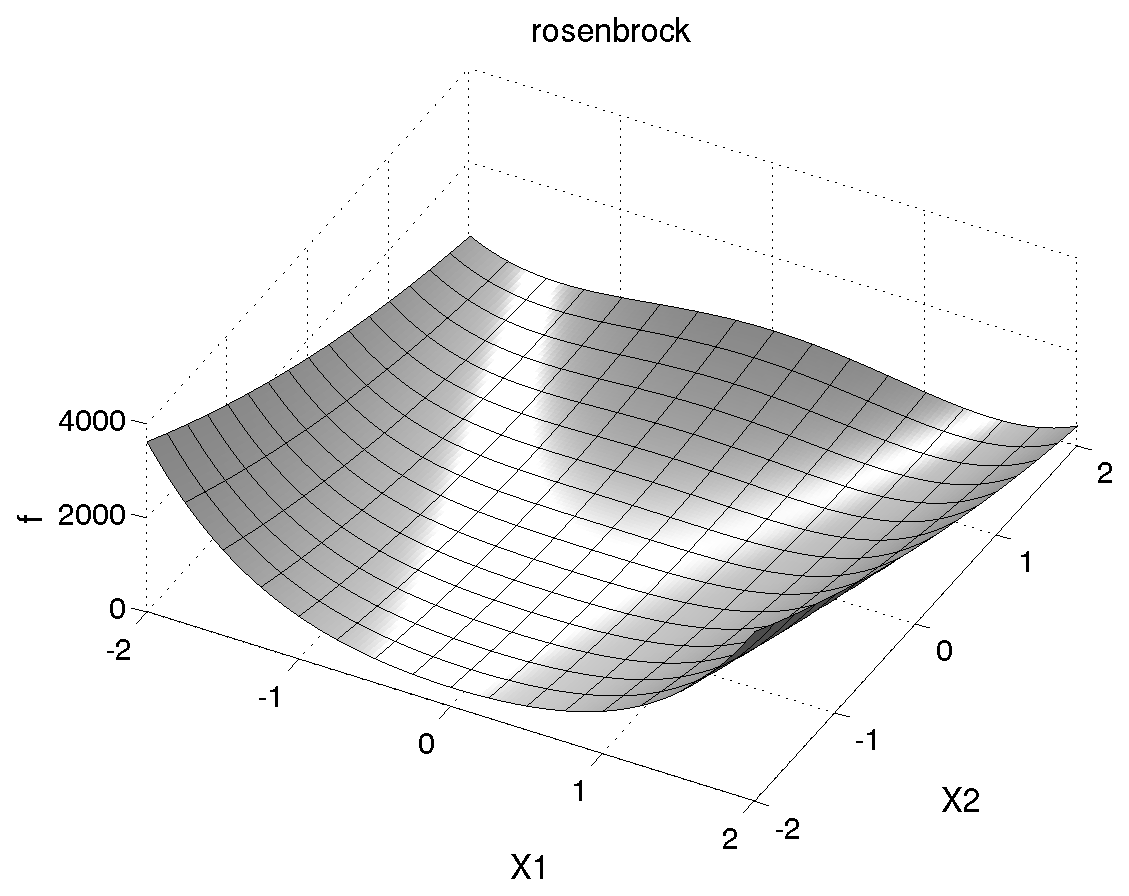
\includegraphics[height=2.5in]{images/rosen_3d_surf} &
  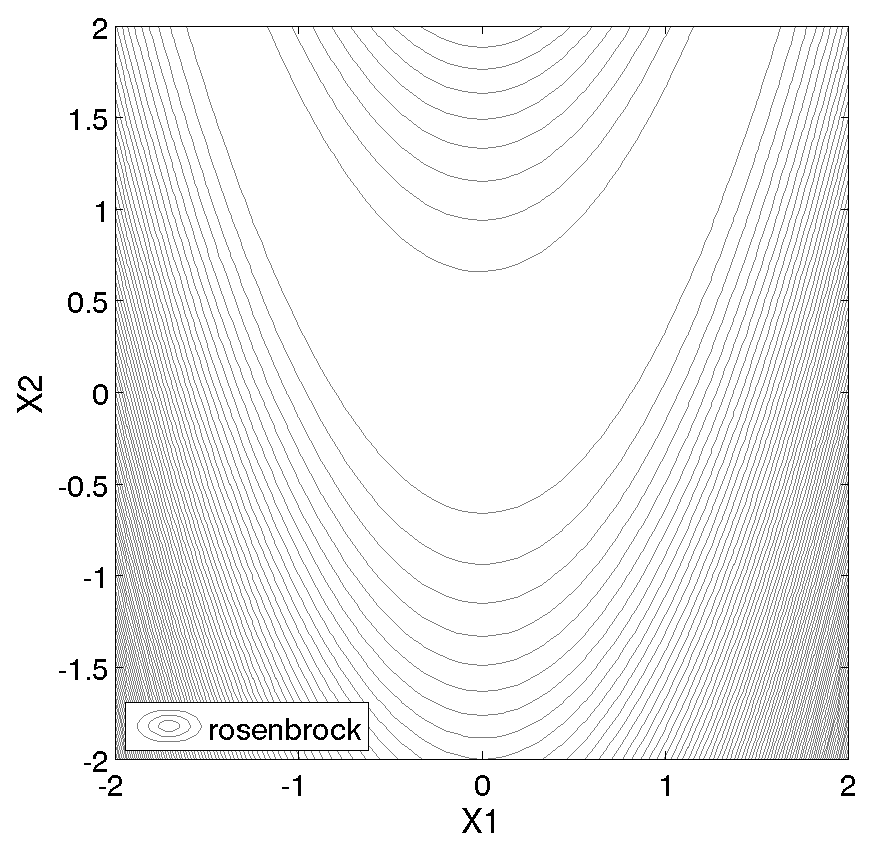
\includegraphics[height=2.5in]{images/rosen_2d_surf} \\
  (a) & (b) \\
  \end{tabular}
  \caption{Rosenbrock's function: (a) 3-D plot and (b) contours with
  $x_1$ on the bottom axis.}
  \label{tutorial:rosenbrock_prob}
\end{figure}

Note that there are no linear or nonlinear constraints in this
formulation, so this is a bound constrained optimization problem. The
unique solution to this problem lies at the point
$(x_1,x_2) = (1,1)$, where the function value is zero.

The two-variable version of the ``textbook'' example problem provides
a nonlinearly constrained optimization test case. It is formulated as:
\begin{eqnarray}
\texttt{minimize }
& & f = (x_1-1)^{4}+(x_2-1)^{4}     \nonumber \\
\texttt{subject to }
& & g_1 = x_1^2-\frac{x_2}{2} \le 0 \nonumber \\
& & g_2 = x_2^2-\frac{x_1}{2} \le 0 \label{tutorial:textbook_f} \\
& &  0.5 \le x_1 \le 5.8            \nonumber \\
& & -2.9 \le x_2 \le 2.9            \nonumber
\end{eqnarray}

Contours of this example problem are illustrated in
Figure~\ref{tutorial:textbook_prob}(a), with a close-up view of
the feasible region given in
Figure~\ref{tutorial:textbook_prob}(b).

\begin{figure}[htp!]
  \centering
  \begin{tabular}{cc}
  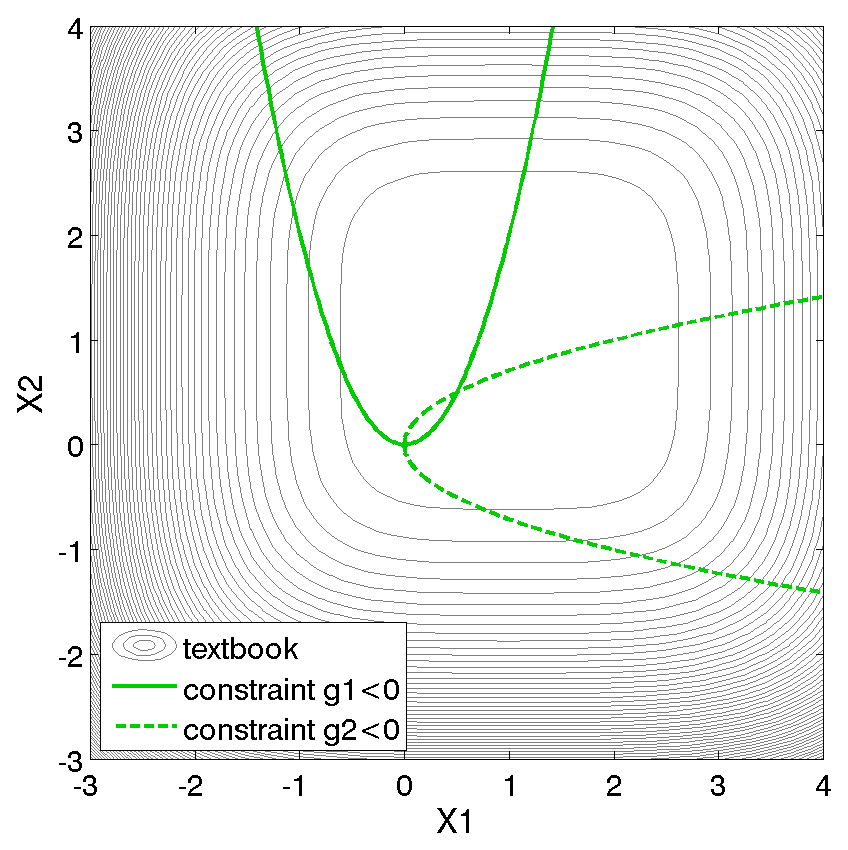
\includegraphics[height=2.5in]{images/textbook_contours} &
  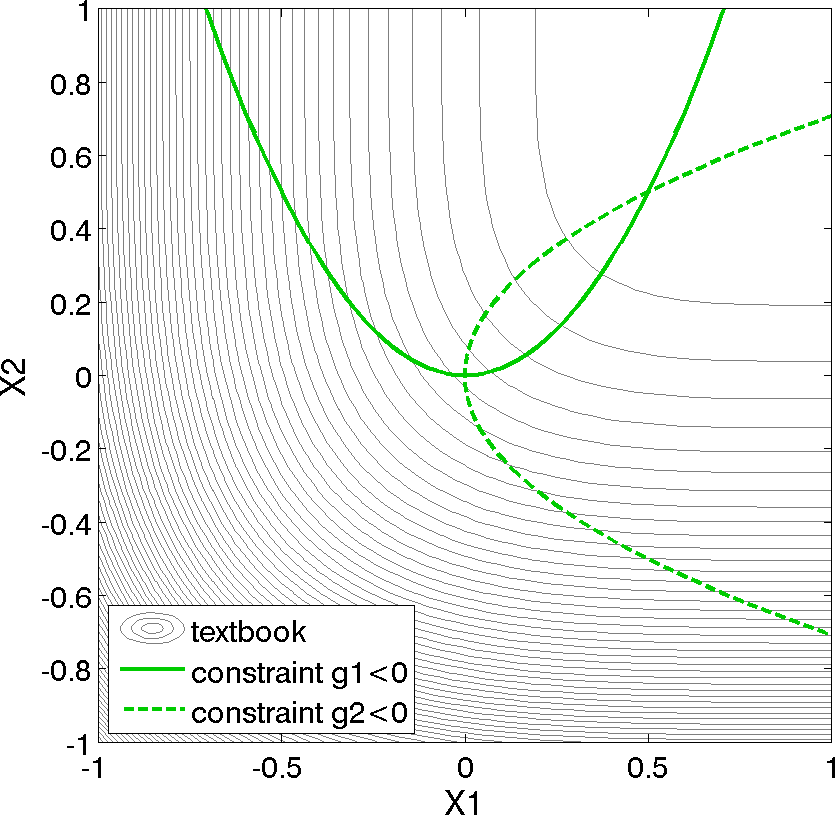
\includegraphics[height=2.5in]{images/textbook_closeup} \\
  (a) & (b) \\
  \end{tabular}
  \caption{Contours of the textbook problem (a) on the $[-3,4] \times
    [-3,4]$ domain and (b) zoomed into an area containing the
    constrained optimum point $(x_1,x_2) = (0.5,0.5)$. The
    feasible region lies at the intersection of the two constraints
    $g_1$ (solid) and $g_2$ (dashed).}
  \label{tutorial:textbook_prob}
\end{figure}

For the textbook example problem, the unconstrained minimum occurs at
$(x_1,x_2) = (1,1)$. However, the inclusion of the constraints
moves the minimum to $(x_1,x_2) = (0.5,0.5)$.

Several other example problems are available. See
Chapter~\ref{additional} for a description of these example problems
as well as further discussion of the Rosenbrock and textbook example
problems.

\section{DAKOTA Input File Format}\label{tutorial:dakota}

All of the DAKOTA input files for the simple example problems
presented here are included in the distribution tar files within
directory \texttt{Dakota/examples/tutorial}. A simple DAKOTA
input file (that is named \texttt{dakota\_rosenbrock\_2d.in})
for a two-dimensional parameter study on Rosenbrock's
function is shown in Figure~\ref{tutorial:rosenbrock_2d}.
This input file will be used to
describe the basic format and syntax used in all DAKOTA input files.

\begin{figure}[ht!]
  \centering
  \begin{bigbox}
    \begin{small}
      \verbatimtabinput[8]{dakota_rosenbrock_2d.in}
    \end{small}
  \end{bigbox}
  \caption{Rosenbrock 2-D parameter study example: the DAKOTA input
    file.}
  \label{tutorial:rosenbrock_2d}
\end{figure}

There are six specification blocks that may appear in DAKOTA input
files. These are identified in the input file using the following
keywords: variables, interface, responses, model, method, and strategy. These
keyword blocks can appear in any order in a DAKOTA input file. At
least one \emph{variables}, \emph{interface}, \emph{responses}, and
\emph{method} specification must appear, and no more than one
\emph{strategy} specification should appear. In Figure~
\ref{tutorial:rosenbrock_2d}, one of each of the keyword blocks is
used.  Additional syntax features include use of the \#
symbol to indicate a comment, use of single or double quotes for string inputs
(e.g., \texttt{'x1'}), the use of commas and/or white space for separation of
specifications, and the optional use of ``='' symbols to indicate
supplied data. See the DAKOTA Reference
Manual~\cite{RefMan} for additional details on this input file syntax.

The first section of the input file shown in
Figure~\ref{tutorial:rosenbrock_2d} is the \emph{strategy} section.
This keyword section is used to specify some of DAKOTA's advanced
meta-procedures such as hybrid optimization, surrogate-based
optimization, multi-start optimization, and Pareto optimization.
See Chapter~\ref{strat} for more information on these
meta-procedures. The \emph{strategy} section also contains the
settings for DAKOTA's graphical output (via the \texttt{graphics}
flag) and the tabular data output (via the
\texttt{tabular\_graphics\_data} keyword).

The \emph{method} section of the input file specifies the iterative
technique that DAKOTA will employ, such as a parameter study,
optimization method, data sampling technique, etc.
The keyword \texttt{multidim\_parameter\_study}
in Figure~\ref{tutorial:rosenbrock_2d} calls for a multidimensional
parameter study, while the keyword \texttt{partitions} specifies the
number of intervals per variable. In this case, there will be eight
intervals (nine data points) evaluated between the lower and upper
bounds of both variables (bounds provided subsequently in the
\emph{variables} section), for a total of 81 response function
evaluations.

The \emph{model} section of the input file specifies the model that
DAKOTA will use.  A model provides the logical unit for determining
how a set of variables is mapped into a set of responses in support of
an iterative method.  The model allows one to specify a single
interface, or to manage more sophisticated mappings involving
surrogates or nested iteration.  For example, one might want to use
an approximate model for optimization or uncertainty quantification,
due to the lower computational cost.  The
\texttt{model} keyword allows one to specify if the iterator will be
operating on a data fit surrogate (such as a polynomial regression,
neural net, etc.), a hierarchical surrogate (which uses the corrected
results of a lower fidelity simulation model as an approximation to a
higher fidelity simulation), or a nested model. See
Chapter~\ref{models} for additional model specification details. If
these advanced facilities for surrogate modeling or nested iteration
are not required, then it is not necessary to specify the
\texttt{model} keyword at all, since the default behavior is the use
of a ``single'' model constructed with the last set of responses,
variables, and interface specified.  In
Figure~\ref{tutorial:rosenbrock_2d}, the keyword \texttt{single}
explicitly specifies the use of a single model in the parameter study,
even though this is the default.

The \emph{variables} section of the input file specifies the
characteristics of the parameters that will be used in the problem
formulation. The variables can be continuous or discrete, and can be
classified as design variables, uncertain variables, or state
variables. See Chapter~\ref{variables} for more information on the
types of variables supported by DAKOTA.  The \emph{variables} section
shown in Figure~\ref{tutorial:rosenbrock_2d} specifies that there are
two continuous design variables.  The sub-specifications for
continuous design variables
% use the abbreviation ``cdv'' in the input file and
provide the descriptors ``x1'' and ``x2'' as well as lower
and upper bounds for these variables. The information about the
variables is organized in column format for readability. So, both
variables $x_1$ and $x_2$ have a lower bound of -2.0 and an upper
bound of 2.0.

The \emph{interface} section of the input file specifies what approach
will be used to map variables into responses as well as details on how
DAKOTA will pass data to and from a simulation code.
In this example, the keyword \texttt{direct} is used to indicate the
use of a function linked directly into DAKOTA.
Alternatively, \texttt{fork} or \texttt{system} executions can be used
to invoke instances of a simulation code that is external to DAKOTA,
as explained in Section \ref{tutorial:example:user_supply:optimization2} 
and Chapter~\ref{advint}.
The \texttt{analysis\_driver} keyword indicates the name of the test
function.  With \texttt{fork} or \texttt{system}, default file names
would be used for passing data between DAKOTA and the simulation code.

The \emph{responses} section of the input file specifies the types of
data that the interface will return to DAKOTA. For the example shown
in Figure~\ref{tutorial:rosenbrock_2d}, the assignment
\texttt{num\_objective\_functions = 1}
indicates that there is only one objective
function.  Since there are no constraints
associated with Rosenbrock's function, the keywords for
constraint specifications are omitted. The keywords
\texttt{no\_gradients} and \texttt{no\_hessians} indicate that no
derivatives will be provided to the method; none are needed for
a parameter study.

\section{Example Problems}\label{tutorial:example}

This section serves to familiarize users without how to perform parameter 
studies, optimization, and uncertainty quantification through their common
DAKOTA interface.  The initial examples utilize simple built in driver 
functions; later we show how to utilize DAKOTA to drive the evaluation of 
user supplied black box code.  The examples presented in this chapter 
are intended to show the simplest use of DAKOTA for several methods of 
each type.  More advanced examples of using DAKOTA for specific purposes 
are provided in subsequent, topic based, chapters.

\subsection{Parameter Studies}\label{tutorial:example:param_study}

Parameter study methods in the DAKOTA toolkit involve the computation 
of response data sets at a selection of points in the parameter space. 
These response data sets are not linked to any specific interpretation,
so they may consist of any allowable specification from the responses 
keyword block, i.e., objective and constraint functions, least squares 
terms and constraints, or generic response functions. This allows the 
use of parameter studies in direct coordination with optimization, least 
squares, and uncertainty quantification studies without significant
modification to the input file.  
The two examples given in this subsection are for a two-dimensional 
tensor product of sample points and a vector parameter study.

\subsubsection{Two-Dimensional Grid Parameter Study}\label{tutorial:example:param_study:two}

The 2-D parameter study example problem listed in Figure~
\ref{tutorial:rosenbrock_2d} is executed by DAKOTA using the
following command:
\begin{small}
\begin{verbatim}
    dakota dakota_rosenbrock_2d.in > 2d.out
\end{verbatim}
\end{small}

The output of the DAKOTA run is directed to the file named
\texttt{2d.out}. For comparison, a file named \texttt{2d.out.sav} is
included in the \texttt{Dakota/examples/tutorial} directory. As
for many of the examples, DAKOTA provides a report on the best design
point located during the study at the end of these output files.

This 2-D parameter study produces the grid of data samples shown in
Figure~\ref{tutorial:rosenbrock_2d_graphics}. In general, a multidimensional 
parameter study lets one generate a grid in multiple dimensions. 
The keyword \texttt{multidim\_parameter\_study} indicates that 
a grid will be generated over all variables.  The keyword 
\texttt{partitions} indicates the number of grid partitions in 
each dimension. For this example, the number of the grid partitions 
are the same in each dimension (8 partitions) but it would be possible 
to specify (partitions = 8 2), and have only two partitions 
over the second input variable.   Note that the
\texttt{graphics} flag in the \emph{strategy} section of the input
file could be commented out since, for this example, the iteration
history plots created by DAKOTA are not particularly instructive. More
interesting visualizations can be created by importing DAKOTA's
tabular data into an external graphics/plotting package. Common
graphics and plotting packages include Mathematica, Matlab, Microsoft
Excel, Origin, Tecplot, and many others. (Sandia National Laboratories
and the DAKOTA developers do not endorse any of these commercial
products.)

\begin{figure}[htb!]
  \centering
  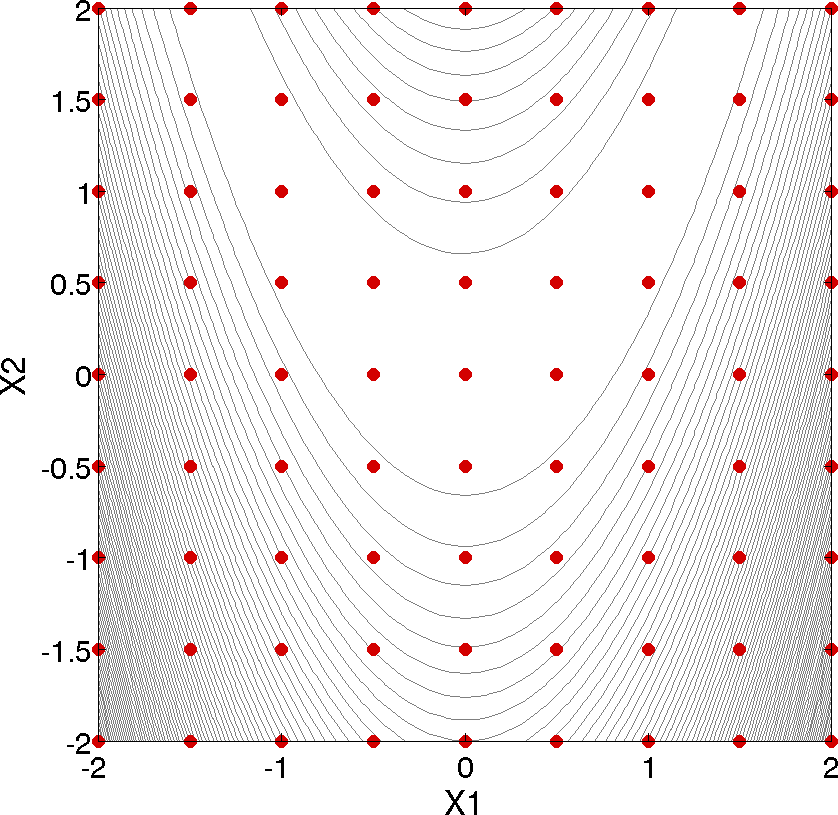
\includegraphics[height=2.5in]{images/rosen_2d_pts}
  \caption{Rosenbrock 2-D parameter study example:
  location of the design points (dots) evaluated.}
  \label{tutorial:rosenbrock_2d_graphics}
\end{figure}

\subsubsection{Vector Parameter Study}\label{tutorial:example:param_study:vector}

In addition to the multidimensional parameter study, DAKOTA can
perform a vector parameter study, i.e., a parameter study between any
two design points in an \emph{n}-dimensional parameter space.

An input file for the vector parameter study is shown in Figure~
\ref{tutorial:rosenbrock_vector}.  The primary differences
between this input file and the previous input file are found in the
\emph{variables} and \emph{method} sections. In the variables section,
the keywords for the bounds are removed and replaced with the keyword
\texttt{initial\_point} that specifies the starting point for the
parameter study. In the method section, the
\texttt{vector\_parameter\_study} keyword is used. The
\texttt{final\_point} keyword indicates the stopping point for the
parameter study, and \texttt{num\_steps} specifies the number of steps
taken between the initial and final points in the parameter study.

\begin{figure}[ht!]
  \centering
  \begin{bigbox}
    \begin{small}
      \verbatimtabinput[8]{dakota_rosenbrock_vector.in}
    \end{small}
  \end{bigbox}
  \caption{Rosenbrock vector parameter study example: the DAKOTA input
  file.}
  \label{tutorial:rosenbrock_vector}
\end{figure}

The vector parameter study example problem is executed using the command
\begin{small}
\begin{verbatim}
    dakota dakota_rosenbrock_vector.in > vector.out
\end{verbatim}
\end{small}

Figure~\ref{tutorial:rosenbrock_vector_graphics}(a) shows the
graphics output created by DAKOTA.  For this study, the simple DAKOTA
graphics are more useful for visualizing the
results. Figure~\ref{tutorial:rosenbrock_vector_graphics}(b)
shows the locations of the 11 sample points generated in this study.
It is evident from these figures that the parameter study starts
within the banana-shaped valley, marches up the side of the hill, and
then returns to the valley. The output file \texttt{vector.out.sav} is
provided in the \texttt{Dakota/examples/tutorial} directory.

In addition to the vector and multidimensional examples shown, DAKOTA
also supports list and centered parameter study methods. Refer to
Chapter~\ref{ps} for additional information.

\begin{figure}[htp!]
  \centering
  \begin{tabular}{c}
  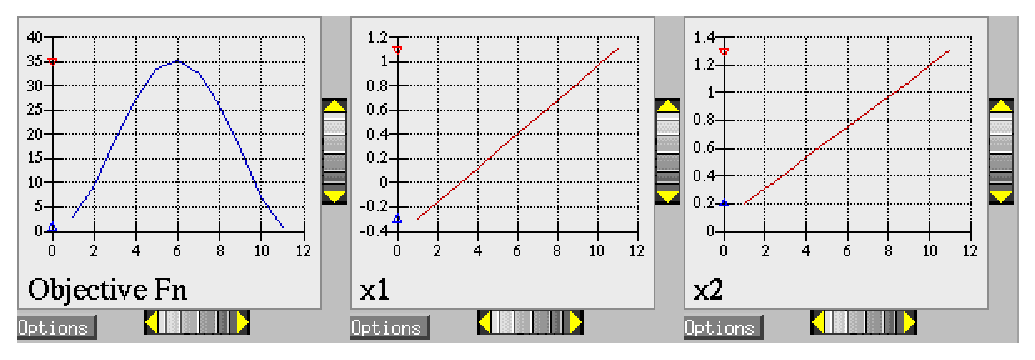
\includegraphics[width=\textwidth]{images/dak_graphics_vector}\\
  (a)\\
  \qquad\\
  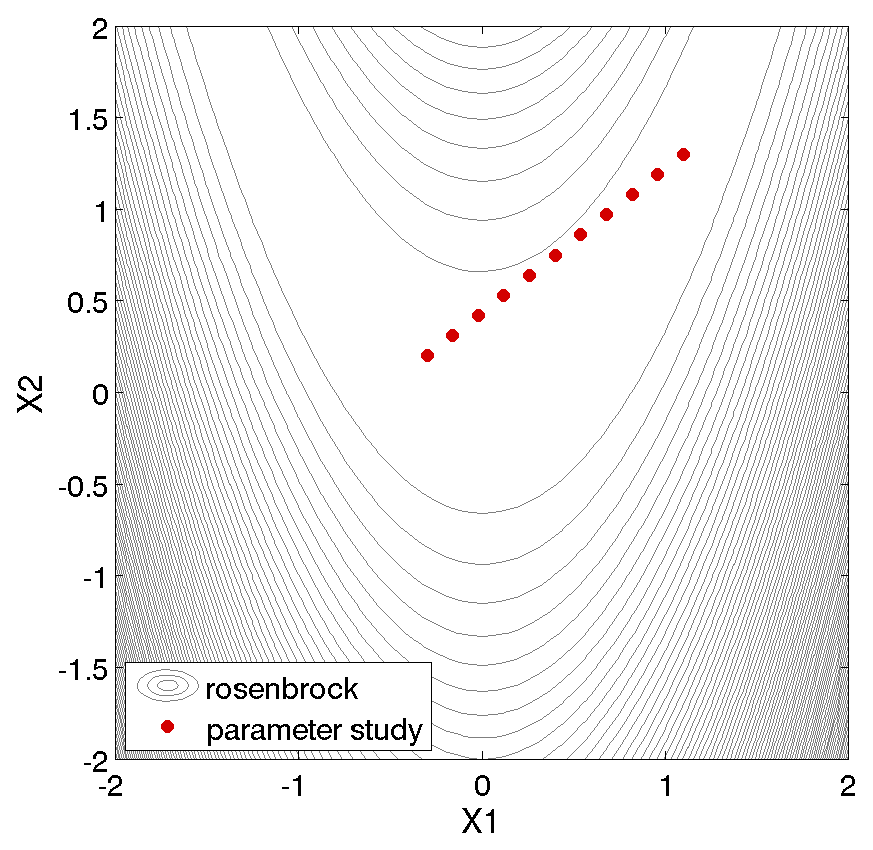
\includegraphics[height=2.5in]{images/rosen_vect_pts} \\
  (b)
  \end{tabular}
  \caption{Rosenbrock vector parameter study example: (a) screen
    capture of the DAKOTA graphics and (b) location of the design
    points (dots) evaluated.}
  \label{tutorial:rosenbrock_vector_graphics}
\end{figure}

\subsection{Optimization}\label{tutorial:example:optimization}

DAKOTA's optimization capabilities include a variety of gradient-based 
and nongradient-based optimization methods. This subsection demonstrates
the use of several such methods through the DAKOTA interface.

\subsubsection{Gradient-based Unconstrained Optimization}\label{tutorial:example:optimization:gradient1}

A DAKOTA input file for a gradient-based optimization of Rosenbrock's
function is listed in Figure~\ref{tutorial:rosenbrock_grad}. The
format of the input file is similar to that used for the parameter
studies, but there are some new keywords in the responses and method
sections.  First, in the responses section of the input file, the
keyword block starting with \texttt{numerical\_gradients} specifies
that a finite difference method will be used to compute gradients for
the optimization algorithm. Note that the Rosenbrock function
evaluation code inside DAKOTA has the ability to give analytical
gradient values.  (To switch from finite difference gradient estimates
to analytic gradients, uncomment the \texttt{analytic\_gradients}
keyword and comment out the four lines associated with the
\texttt{numerical\_gradients} specification.)
Next, in the method
section of the input file, several new keywords have been added. In
this section, the keyword \texttt{conmin\_frcg} indicates the use of
the Fletcher-Reeves conjugate gradient algorithm in the CONMIN
optimization software package~\cite{Van78} for bound-constrained
optimization.  The keyword \texttt{max\_iterations} is used to
indicate the computational budget for this optimization (in this case,
a single iteration includes multiple evaluations of Rosenbrock's
function for the gradient computation steps and the line search
steps). The keyword \texttt{convergence\_tolerance} is used to specify
one of CONMIN's convergence criteria (under which CONMIN terminates if the
objective function value differs by less than the absolute value of
the convergence tolerance for three successive iterations).
% And, finally, the \texttt{output} verbosity is set to \texttt{quiet}.

\begin{figure}
  \centering
  \begin{bigbox}
    \begin{small}
      \verbatimtabinput[8]{dakota_rosenbrock_grad_opt.in}
    \end{small}
  \end{bigbox}
  \caption{Rosenbrock gradient-based unconstrained optimization
  example: the DAKOTA input file.}
  \label{tutorial:rosenbrock_grad}
\end{figure}

This DAKOTA input file is executed using the following command:
\begin{small}
\begin{verbatim}
    dakota dakota_rosenbrock_grad_opt.in > grad_opt.out
\end{verbatim}
\end{small}

The sample file \texttt{grad\_opt.out.sav} is included in
\texttt{Dakota/examples/tutorial} for comparison. When this
example problem is executed, DAKOTA creates some iteration history
graphics similar to the screen capture shown in Figure~
\ref{tutorial:rosenbrock_grad_graphics}(a). These plots show
how the objective function and design parameters change in value
during the optimization steps. The scaling of the horizontal and
vertical axes can be changed by moving the scroll knobs on each plot.
Also, the ``Options'' button allows the user to plot the vertical axes
using a logarithmic scale.  Note that log-scaling is only allowed if
the values on the vertical axis are strictly greater than zero.

\begin{figure}[ht!]
  \centering
  \begin{tabular}{c}
  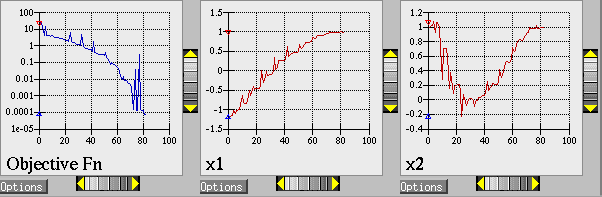
\includegraphics[width=\textwidth]{images/dak_graphics_grad_opt}\\
  (a)\\
  \qquad\\
  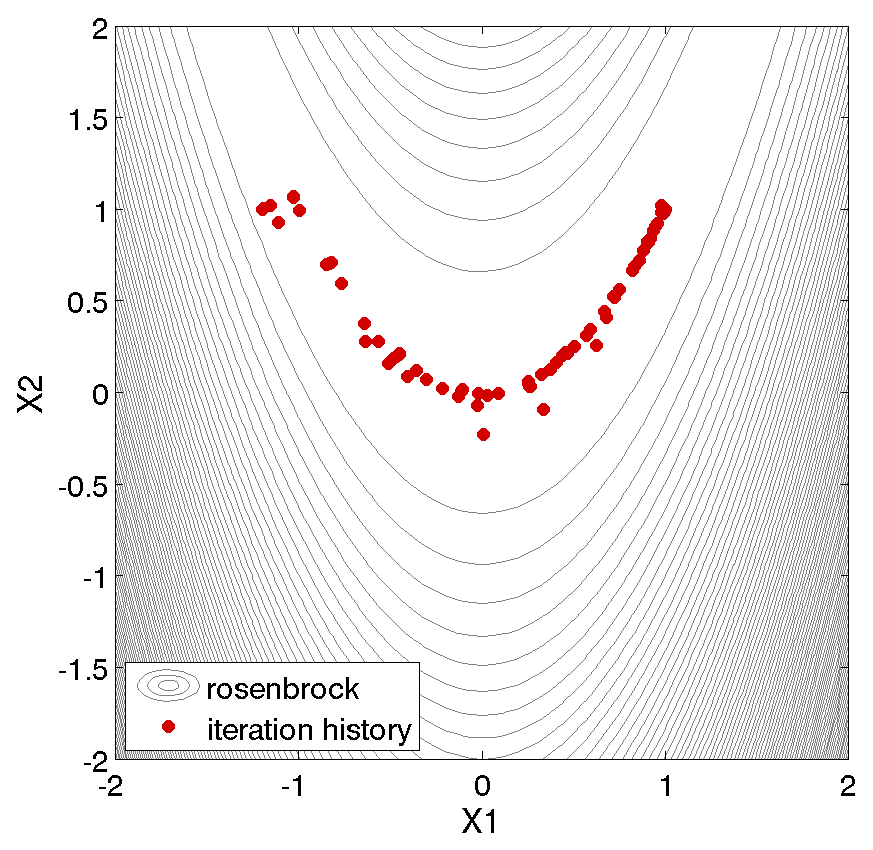
\includegraphics[height=2.5in]{images/rosen_grad_opt_pts} \\
  (b)
  \end{tabular}
  \caption{Rosenbrock gradient-based unconstrained optimization
    example: (a) screen capture of the DAKOTA graphics and (b)
    sequence of design points (dots) evaluated (line search points
    omitted).}
  \label{tutorial:rosenbrock_grad_graphics}
\end{figure}

Figure~\ref{tutorial:rosenbrock_grad_graphics}(b) shows the
iteration history of the optimization algorithm.  The optimization
starts at the point $(x_1,x_2) = (-1.2,1.0)$ as given in the
DAKOTA input file.  Subsequent iterations follow the banana-shaped
valley that curves around toward the minimum point at $(x_1,x_2) =
(1.0,1.0)$. Note that the function evaluations associated with the
line search phase of each CONMIN iteration are not shown on the plot.
At the end of the DAKOTA run, information is written to the output
file to provide data on the optimal design point. These data include
the optimum design point parameter values, the optimum objective and
constraint function values (if any), plus the number of function
evaluations that occurred and the amount of time that elapsed during
the optimization study.

\subsubsection{Gradient-based Constrained Optimization}\label{tutorial:example:gradient2}

This example demonstrates the use of a gradient-based optimization
algorithm on a nonlinearly constrained problem. The ``textbook''
example problem (see Section~\ref{tutorial:rosenbrock}) is used
for this purpose and the DAKOTA input file for this example problem is
shown in Figure~\ref{tutorial:textbook_grad_constr}.  This
input file is similar to the input file for the unconstrained
gradient-based optimization example problem involving the Rosenbrock
function.  Note the addition of commands in the responses section of
the input file that identify the number and type of constraints, along
with the upper bounds on these constraints.  The commands
\texttt{direct} and \texttt{analysis\_driver = 'text\_book'} specify
that DAKOTA will use its internal version of the textbook problem.

\begin{figure}[ht!]
  \centering
  \begin{bigbox}
    \begin{small}
      \verbatimtabinput[8]{dakota_textbook.in}
    \end{small}
  \end{bigbox}
  \caption{Textbook gradient-based constrained optimization example:
    the DAKOTA input file.}
  \label{tutorial:textbook_grad_constr}
\end{figure}

The following command runs this example problem:
\begin{small}
\begin{verbatim}
    dakota dakota_textbook.in > textbook.out
\end{verbatim}
\end{small}

The \texttt{conmin\_mfd} keyword in Figure~\ref{tutorial:textbook_grad_constr} 
tells DAKOTA to use the CONMIN package's implementation of the
Method of Feasible Directions (see Section~\ref{opt:software:conmin} 
for more details).  A significantly faster alternative is the DOT package's 
Modified Method of Feasible Directions, i.e. \texttt{dot\_mmfd} (see 
Section~\ref{opt:software:dot} for more details).  However, DOT is 
licensed software that may not be available on a particular system.  If it 
is installed on your system and DAKOTA has been compiled without the 
\texttt{--without-dot} flag, you may use it by commenting out the line with
\texttt{conmin\_mfd} and uncommenting the line with \texttt{dot\_mmfd}.

The file \texttt{textbook.out.sav} is included in
\texttt{Dakota/examples/tutorial} for comparison purposes. The
results of the optimization example problem are listed at the end of
the \texttt{textbook.out} file. This information shows that the
optimizer stopped at the point $(x_1,x_2) = (0.5,0.5)$, where both
constraints are approximately satisfied, and where the objective function value is
$0.128$. The progress of the optimization algorithm is shown in
Figure~\ref{tutorial:textbook_grad_constr_graphics}(a) where the
dots correspond to the end points of each iteration in the algorithm.  The
starting point is $(x_1,x_2) = (0.9,1.1)$, where both constraints
are violated. The optimizer takes a
sequence of steps to minimize the objective function while reducing
the infeasibility of the constraints.
The optimization graphics are also shown in
Figure~\ref{tutorial:textbook_grad_constr_graphics}(b).

\begin{figure}[ht!]
  \centering
  \begin{tabular}{c}
  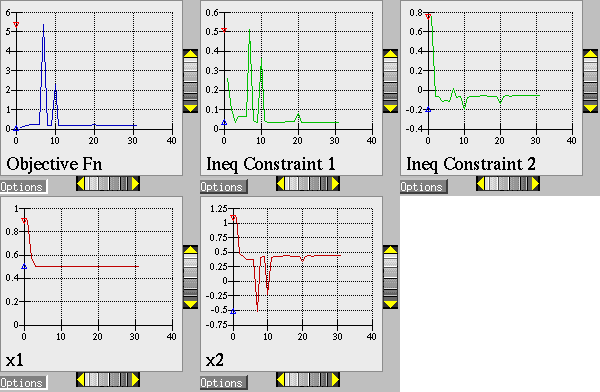
\includegraphics[width=\textwidth]{images/textbook_opt_hist}\\
  (a)\\
  \qquad\\
  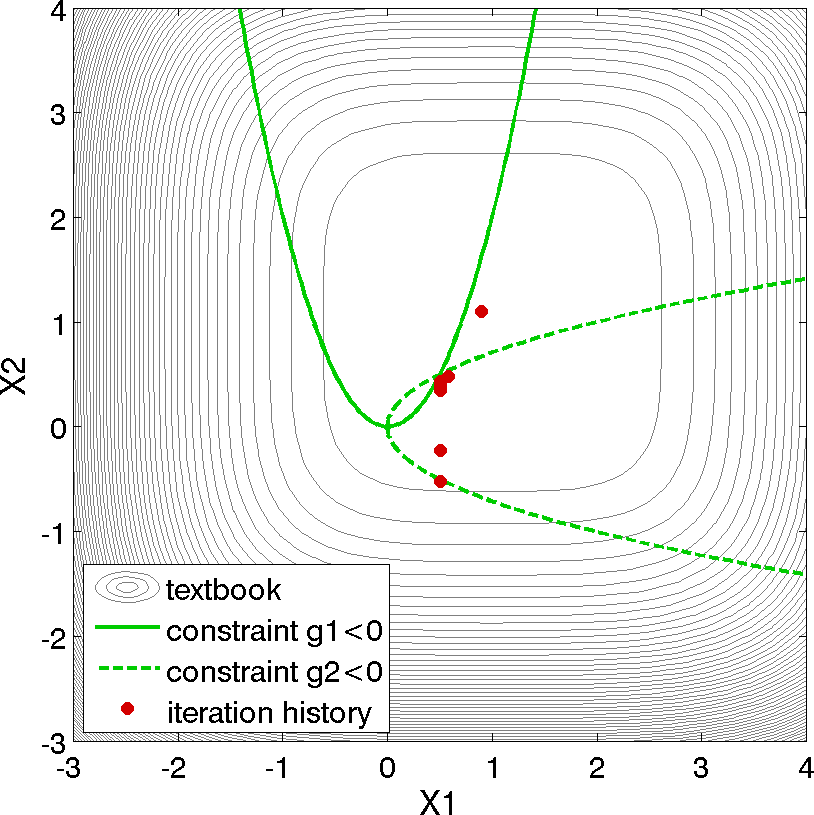
\includegraphics[height=2.5in]{images/textbook_history} \\
  (b)
  \end{tabular}
  \caption{Textbook gradient-based constrained optimization example:
    (a) screen capture of the DAKOTA graphics shows how the objective
    function was reduced during the search for a feasible design point
    and (b) iteration history (iterations marked by solid dots).}
  \label{tutorial:textbook_grad_constr_graphics}
\end{figure}

%\newpage
\subsubsection{Nonlinear Least Squares Methods for Optimization}\label{tutorial:example:nonlinear}

Both the Rosenbrock and textbook example problems can be formulated as
least-squares minimization problems (see
Section~\ref{additional:textbook} and
Section~\ref{additional:rosenbrock}). For example, the Rosenbrock
problem can be cast as:
\begin{equation}
\texttt{minimize } (f_1)^2 + (f_2)^2
\end{equation}

where $f_1 = 10(x_2-x_1^2)$ and $f_2 = (1-x_1)$. When
using a least-squares approach to minimize a function, each of the
least-squares terms $f_1, f_2,\ldots$ is driven toward zero. This
formulation permits the use of specialized algorithms that can be more
efficient than general purpose optimization algorithms. See
Chapter~\ref{nls} for more detail on the algorithms used for least-squares
minimization, as well as a discussion on the types of
engineering design problems (e.g., parameter estimation) that can make
use of the least-squares approach.

Figure~\ref{tutorial:rosenbrock_nls} is a listing of the DAKOTA input
file \texttt{dakota\_rosenbrock\_ls.in}. This input file differs from
the input file shown in Figure~\ref{tutorial:rosenbrock_grad} in
several key areas. The responses section of the input file uses the
keyword \texttt{num\_least\_squares\_terms = 2} instead of the
\texttt{num\_objective\_functions = 1}.
%The keywords in the interface section show that the Unix fork method
%is used to run the C++ analysis code named \texttt{rosenbrock}.
The method section of the input file shows that the NL2SOL
algorithm~\cite{Den81} (\texttt{nl2sol}) is used in this example.  (The
Gauss-Newton, NL2SOL, and NLSSOL SQP algorithms are currently
available for exploiting the special mathematical structure of least
squares minimization problems).

\begin{figure}[ht!]
  \centering
  \begin{bigbox}
    \begin{small}
      \verbatimtabinput[8]{dakota_rosenbrock_ls.in}
    \end{small}
  \end{bigbox}
  \caption{Rosenbrock nonlinear least squares example: the DAKOTA input file.}
  \label{tutorial:rosenbrock_nls}
\end{figure}

The input file listed in Figure~\ref{tutorial:rosenbrock_nls} is
executed using the command:
\begin{small}
\begin{verbatim}
    dakota dakota_rosenbrock_ls.in > leastsquares.out
\end{verbatim}
\end{small}

The file \texttt{leastsquares.out.sav} is included
\texttt{Dakota/examples/tutorial} for comparison purposes. The
optimization results at the end of this file show that the least
squares minimization approach has found the same optimum design point,
$(x1,x2) = (1.0,1.0)$, as was found using the conventional
gradient-based optimization approach. The iteration history of the
least squares minimization is given in
Figure~\ref{tutorial:rosenbrock_nls_graphics}, and shows that 14
function evaluations were needed for convergence. In this example the
least squares approach required about half the number of function
evaluations as did conventional gradient-based optimization.
In many cases a good least squares algorithm will converge more rapidly
in the vicinity of the solution.

\begin{figure}[ht!]
  \centering
  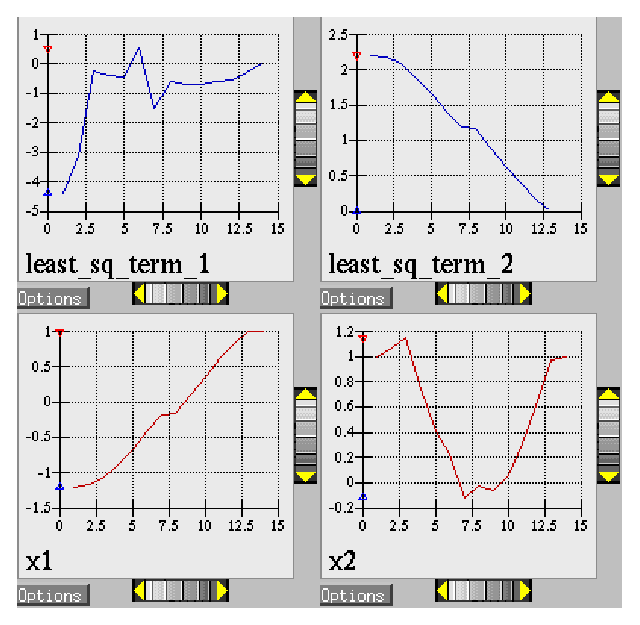
\includegraphics[height=4in]{images/nonlin_paramest_hist}
  \caption{Rosenbrock nonlinear least squares example: iteration
    history for least squares terms $f_1$ and $f_2$.}
  \label{tutorial:rosenbrock_nls_graphics}
\end{figure}

\subsubsection{Nongradient-based Optimization via Pattern Search}\label{tutorial:example:optimization:nongradient1}

In addition to gradient-based optimization algorithms, DAKOTA also
contains a variety of nongradient-based algorithms. One particular
nongradient-based algorithm for local optimization is known as pattern
search (see Chapter~\ref{introduction} for a discussion of local
versus global optimization). The DAKOTA input file shown in
Figure~\ref{tutorial:rosenbrock_patternsearch} applies a pattern
search method to minimize the Rosenbrock function.  While this
provides for an interesting comparison to the previous example
problems in this chapter, the Rosenbrock function is not the best test
case for a pattern search method. That is, pattern search methods are
better suited to problems where the gradients are too expensive to
evaluate, inaccurate, or nonexistent --- situations common among many
engineering optimization problems. It also should be noted that
nongradient-based algorithms generally are applicable only to
unconstrained or bound-constrained optimization problems, although the
inclusion of general linear and nonlinear constraints in
nongradient-based algorithms is an active area of research in the
optimization community. For most users who wish to use
nongradient-based algorithms on constrained optimization problems, the
easiest route is to create a penalty function, i.e., a composite
function that contains the objective function and the constraints,
external to DAKOTA and then optimize on this penalty function. Most
optimization textbooks will provide guidance on selecting and using
penalty functions.

The DAKOTA input file shown in
Figure~\ref{tutorial:rosenbrock_patternsearch} is similar to the
input file for the gradient-based optimization, except it has a
different set of keywords in the method section of the input file, and
the gradient specification in the responses section has been changed
to \texttt{no\_gradients}. The pattern search optimization algorithm
used is part of the COLINY library~\cite{Har06}.  See the DAKOTA
Reference Manual~\cite{RefMan} for more information on the
\emph{methods} section commands that can be used with COLINY
algorithms.

\begin{figure}[ht!]
  \centering
  \begin{bigbox}
    \begin{small}
      \verbatimtabinput[8]{dakota_rosenbrock_ps_opt.in}
    \end{small}
  \end{bigbox}
  \caption{Rosenbrock pattern search optimization example: the DAKOTA input file.}
  \label{tutorial:rosenbrock_patternsearch}
\end{figure}

This DAKOTA input file is executed using the following command:
\begin{small}
\begin{verbatim}
    dakota dakota_rosenbrock_ps_opt.in > ps_opt.out
\end{verbatim}
\end{small}

The file \texttt{ps\_opt.out.sav} is included in the
\texttt{Dakota/examples/tutorial} directory. For this run, the
optimizer was given an initial design point of $(x_1,x_2)
  = (0.0,0.0)$ and was limited to 2000 function evaluations. In this
case, the pattern search algorithm stopped short of the optimum at
$(x_1,x_2) = (1.0,1,0)$, although it was making progress
in that direction when it was terminated.  (It would have
reached the minimum point eventually.)

The iteration history is provided in Figures~
\ref{tutorial:rosenbrock_patternsearch_graphics}(a) and (b), which show
the locations of the function evaluations used in the pattern search
algorithm.
Figure~\ref{tutorial:rosenbrock_patternsearch_graphics}(c)
provides a close-up view of the pattern search function evaluations
used at the start of the algorithm. The coordinate pattern is clearly
visible at the start of the iteration history, and the decreasing size
of the coordinate pattern is evident at the design points move toward
$(x_1,x_2) = (1.0,1.0)$.

\begin{figure}[ht!]
  \centering
  \begin{tabular}{cc}
  \multicolumn{2}{c}
	      {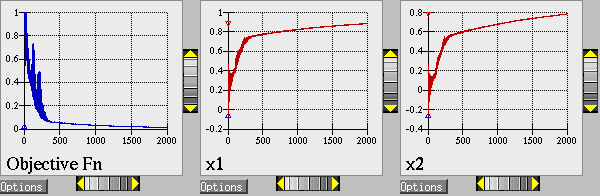
\includegraphics[width=\textwidth]{images/dak_graphics_ps_opt}}\\
  \multicolumn{2}{c}{(a)}\\
  \qquad\\
  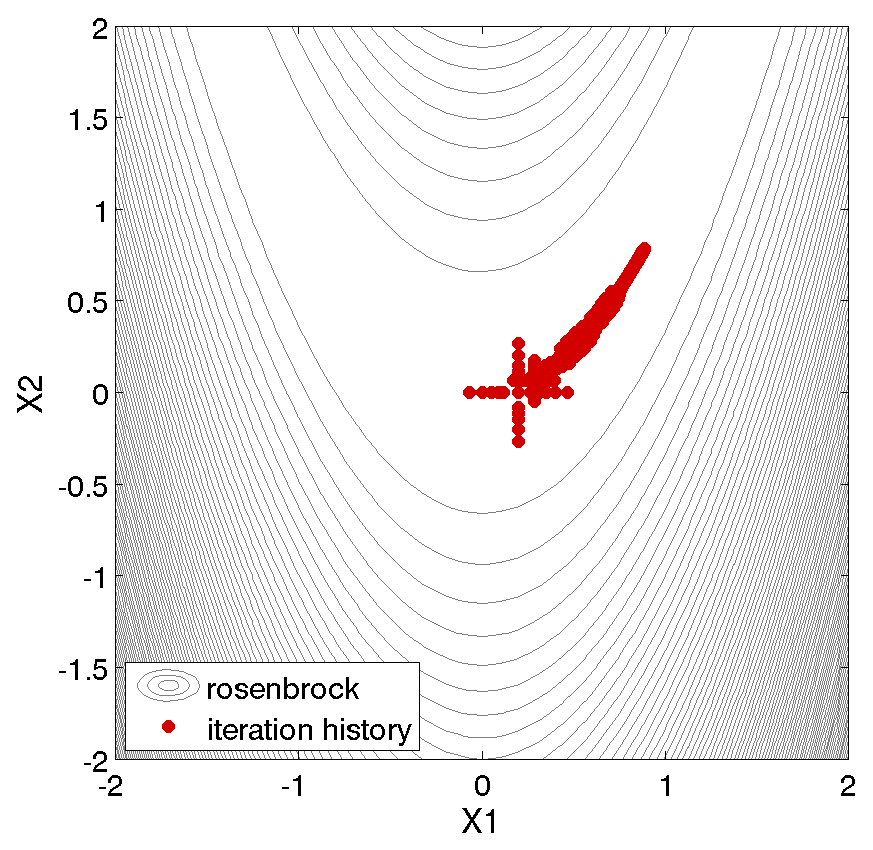
\includegraphics[height=2.5in]{images/rosen_ps_opt_pts} &
  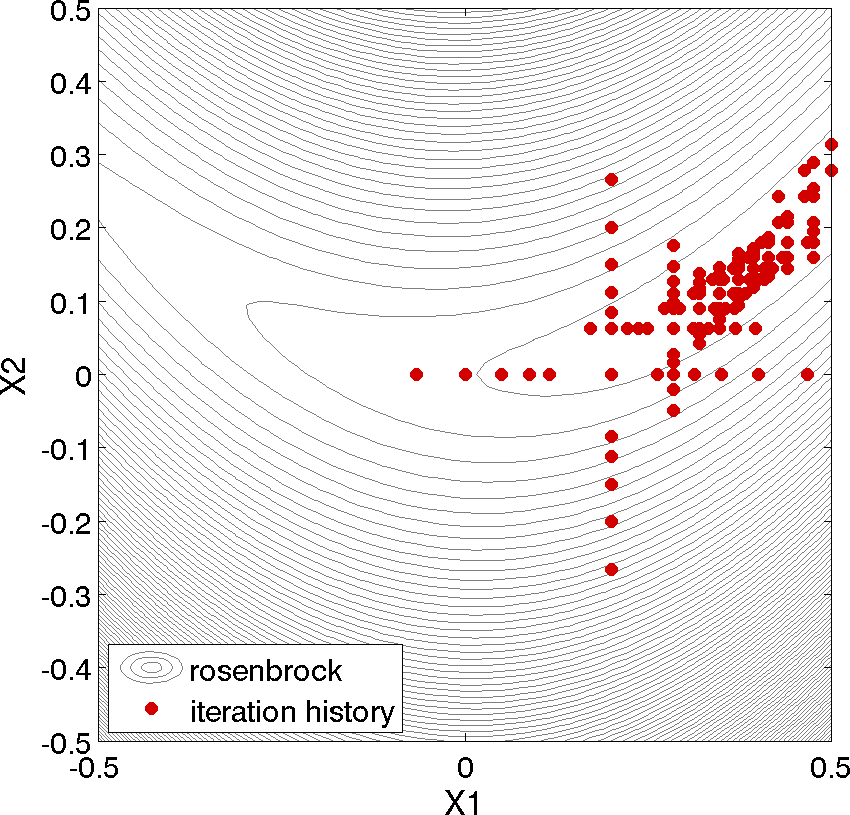
\includegraphics[height=2.5in]{images/rosen_ps_opt_pts2} \\
  (b) & (c)
  \end{tabular}
  \caption{Rosenbrock pattern search optimization example: (a) screen
    capture of the DAKOTA graphics, (b) sequence of design points
    (dots) evaluated and (c) close-up view illustrating the shape of
    the coordinate pattern used. }
  \label{tutorial:rosenbrock_patternsearch_graphics}
\end{figure}

While pattern search algorithms are useful in many optimization
problems, this example shows some of the drawbacks to this algorithm.
While a pattern search method may make good initial progress towards
an optimum, it is often slow to converge. On a smooth, differentiable
function such as Rosenbrock's function, a nongradient-based method
will not be as efficient as a gradient-based method. However, there
are many engineering design applications where gradient information is
inaccurate or unavailable, which renders gradient-based optimizers
ineffective. Thus, pattern search algorithms (and other
nongradient-based algorithms such as genetic algorithms as discussed in the
next section) are often good choices in complex engineering applications
when the quality of gradient data is suspect.

\subsubsection{Nongradient-based Optimization via Evolutionary Algorithm}\label{tutorial:example:optimization:nongradient2}

In contrast to pattern search algorithms, which are local optimization
methods, evolutionary algorithms (EA) are global optimization
methods. As was described above for the pattern search algorithm, the
Rosenbrock function is not an ideal test problem for showcasing the
capabilities of evolutionary algorithms. Rather, EAs are best suited
to optimization problems that have multiple local optima, and where
gradients are either too expensive to compute or are not readily available.

Evolutionary algorithms are based on Darwin's theory of survival of
the fittest. The EA algorithm starts with a randomly selected
population of design points in the parameter space, where the values
of the design parameters form a ``genetic string,'' analogous
to DNA in a biological system, that uniquely represents each design
point in the population. The EA then follows a sequence of
generations, where the best design points in the population (i.e.,
those having low objective function values) are considered to be the
most ``fit'' and are allowed to survive and reproduce. The EA
simulates the evolutionary process by employing the mathematical
analogs of processes such as natural selection, breeding, and
mutation. Ultimately, the EA identifies a design point (or a family of
design points) that minimizes the objective function of the
optimization problem. An extensive discussion of EAs is beyond the
scope of this text, but may be found in a variety of sources (cf.,
~\cite{Haf92} pp. 149-158;~\cite{Gol89}). Currently, the EAs available
in DAKOTA include a genetic algorithm for problems involving discrete
variables and an evolution strategy with self-adaptation for problems
with continuous variables. Details of these algorithms are given in
the DAKOTA Reference Manual~\cite{RefMan}. The COLINY library, which
provides the EA software that has been linked into DAKOTA, is
described in~\cite{Har06}.

\begin{figure}[ht!]
  \centering
  \begin{bigbox}
    \begin{small}
      \verbatimtabinput[8]{dakota_rosenbrock_ea_opt.in}
    \end{small}
  \end{bigbox}
  \caption{Rosenbrock evolutionary algorithm optimization example: the
  DAKOTA input file.}
  \label{tutorial:rosenbrock_ea}
\end{figure}

Figure~\ref{tutorial:rosenbrock_ea} shows a DAKOTA input file that
uses an EA to minimize the Rosenbrock function. For this
example the EA has a population size of 50. At the start of the first
generation, a random number generator is used to select 50 design
points that will comprise the initial population. \emph{[A specific
  seed value is used in this example to generate repeatable results,
  although, in general, one should use the default setting which
  allows the EA to choose a random seed.]} A two-point crossover
technique is used to exchange genetic string values between the
members of the population during the EA breeding process. The result
of the breeding process is a population comprised of the 10 best
``parent'' design points (elitist strategy) plus 40 new ``child''
design points. The EA optimization process will be terminated after
either 100 iterations (generations of the EA) or 2,000 function
evaluations. The EA software available in DAKOTA provides the user
with much flexibility in choosing the settings used in the
optimization process. See~\cite{RefMan} and~\cite{Har06} for details on these
settings.

The following command runs DAKOTA on the input file:
\begin{small}
\begin{verbatim}
    dakota dakota_rosenbrock_ea_opt.in > ea_opt.out
\end{verbatim}
\end{small}

A corresponding output file named \texttt{ea\_opt.out.sav} appears in
\texttt{Dakota/examples/tutorial}. The EA optimization results
printed at the end of this file show that the best design point found
was $(x_1,x_2) = (0.98,0.95)$. The file
\texttt{ea\_tabular.dat.sav} provides a listing of the design
parameter values and objective function values for all 2,000 design
points evaluated during the running of the EA.  Figure~
\ref{tutorial:rosenbrock_ea_graphics}(a) shows the population of
50 randomly selected design points that comprise the first generation
of the EA, and Figure~\ref{tutorial:rosenbrock_ea_graphics}(b)
shows the final population of 50 design points, where most of the 50
points are clustered near $(x_1,x_2) = (0.98,0.95)$.

\begin{figure}[hbt!]
  \centering
  \begin{tabular}{cc}
  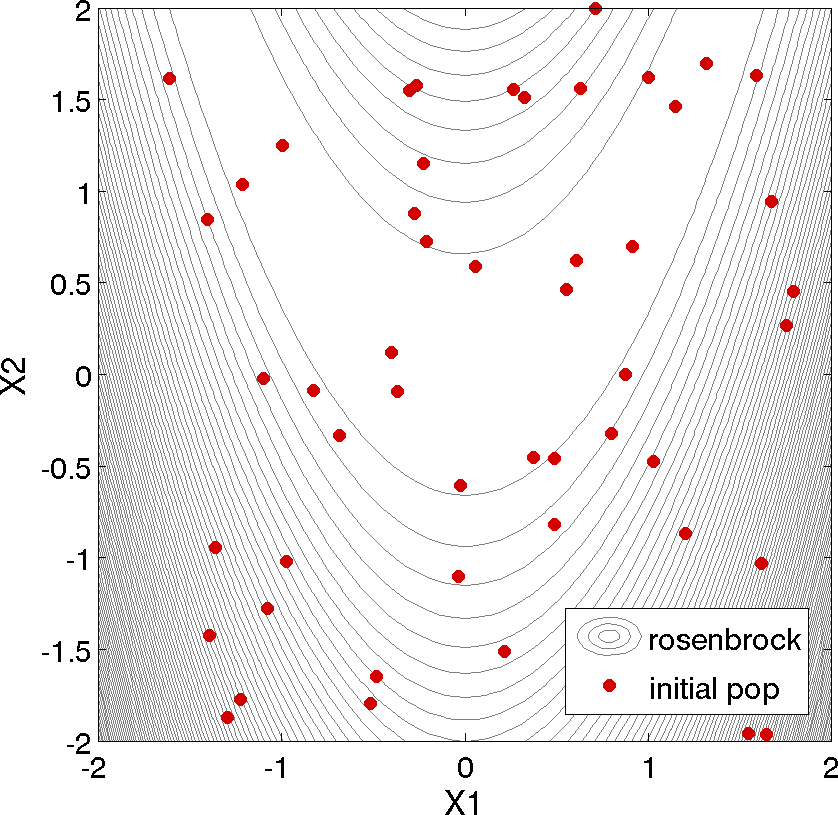
\includegraphics[height=2.5in]{images/rosen_ea_init} &
  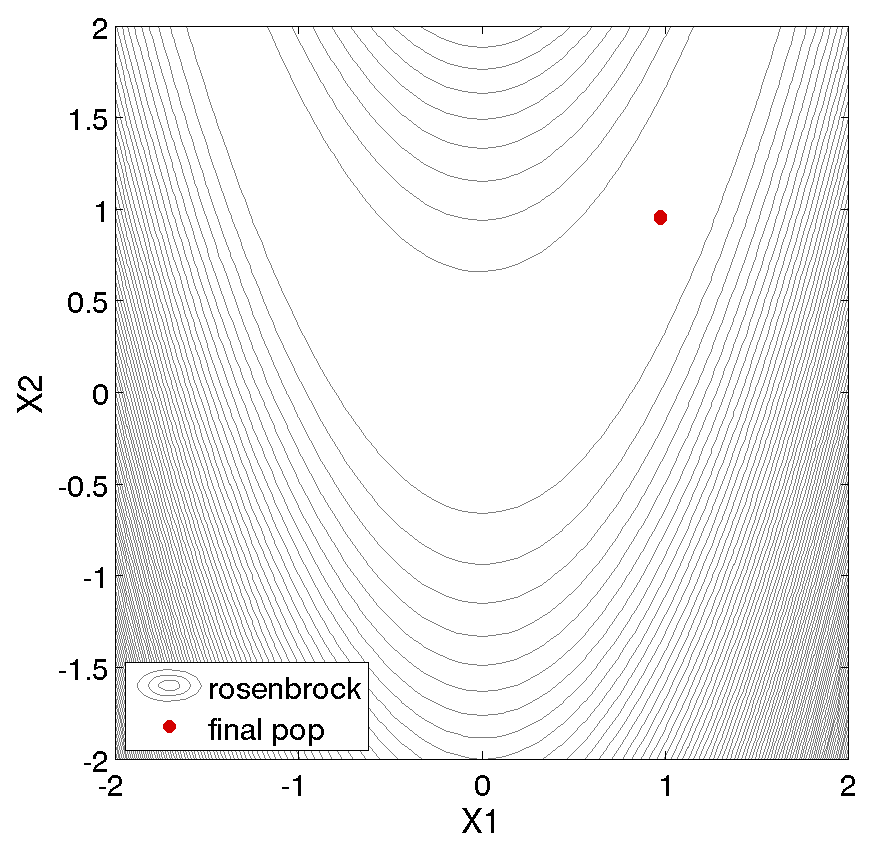
\includegraphics[height=2.5in]{images/rosen_ea_final} \\
  (a) & (b)
  \end{tabular}
  \caption{Rosenbrock evolutionary algorithm optimization example: 50
    design points in the (a) initial and (b) final populations
    selected by the evolutionary algorithm. }
  \label{tutorial:rosenbrock_ea_graphics}
\end{figure}

As described above, an EA is not well-suited to an optimization
problem involving a smooth, differentiable objective such as the
Rosenbrock function. Rather, EAs are better suited to optimization
problems where conventional gradient-based optimization fails, such as
situations where there are multiple local optima and/or gradients are
not available. In such cases, the computational expense of an EA is
warranted since other optimization methods are not applicable or
impractical. In many optimization problems, EAs often quickly identify
promising regions of the design space where the global minimum may be
located. However, an EA can be slow to converge to the optimum. For
this reason, it can be an effective approach to combine the global
search capabilities of a EA with the efficient local search of a
gradient-based algorithm in a \emph{hybrid optimization} strategy.  In
this approach, the optimization starts by using a few iterations of a
EA to provide the initial search for a good region of the parameter
space (low objective function and/or feasible constraints), and then
it switches to a gradient-based algorithm (using the best design point
found by the EA as its starting point) to perform an efficient local
search for an optimum design point. More information on this hybrid
approach is provided in Chapter~\ref{strat}.

In addition to the evolutionary algorithm capabilities in the
\texttt{coliny\_ea} method, there is a single-objective genetic algorithm
method called \texttt{soga}.
%The major differences are that
%\texttt{soga} allows a warm start (e.g., you can read in starting
%solutions from a file), and it allows one to specify a mix of
%continuous and discrete design variables.
For more information on \texttt{soga}, see Chapter~\ref{opt}.

\subsubsection{Multiobjective Optimization}\label{tutorial:example:optimization:multiobjective}

Multiobjective optimization means that there are two or more
objective functions that you wish to optimize simultaneously.  Often
these are conflicting objectives, such as cost and performance.  The
answer to a multi-objective problem is usually not a single point.
Rather, it is a set of points called the Pareto front.  Each point
on the Pareto front satisfies the Pareto optimality criterion, i.e.,
locally there exists no other feasible vector that would improve some
objective without causing a simultaneous worsening in at least one
other objective.  Thus a feasible point $X^\prime$ from which
small moves improve one or more objectives without worsening
any others is not Pareto optimal: it is said to be ``dominated''
and the points along the Pareto front are said to be
``non-dominated''.

Often multi-objective problems are addressed by simply assigning
weights to the individual objectives, summing the weighted
objectives, and turning the problem into a single-objective one
which can be solved with a variety of optimization techniques. While
this approach provides a useful ``first cut'' analysis (and is
supported within DAKOTA---see Section~\ref{opt:additional}), this
approach has many limitations.  The major limitation is that a
local solver with a weighted sum objective will only find one
% optimal solutions if the true Pareto front is nonconvex. %Hogwash!
point on the Pareto front; if one wants to understand
the effects of changing weights, this method can be computationally
expensive.  Since each optimization of a single weighted objective
will find only one point on the Pareto front, many
optimizations must be performed to get a good parametric
understanding of the influence of the weights and to achieve a good
sampling of the entire Pareto frontier.

Starting with version 3.2 of DAKOTA, a capability to perform
multi-objective optimization based on a genetic algorithm method has
been available.  This method is called \texttt{moga}.  It is based on
the idea that as the population evolves in a GA, solutions that are
non-dominated are chosen to remain in the population.  Until version
4.0 of DAKOTA, there was a selection\_type choice of domination\_count
that performed a custom fitness assessment and selection operation
together.  As of version 4.0 of DAKOTA, that functionality has been
broken into separate, more generally usable fitness assessment and
selection operators called the domination\_count fitness assessor and
below\_limit selector respectively.  The effect of using these two
operators is the same as the previous behavior of the
domination\_count selector.  This means of selection works especially
well on multi-objective problems because it has been specifically
designed to avoid problems with aggregating and scaling objective
function values and transforming them into a single
objective. Instead, the fitness assessor works by ranking population
members such that their resulting fitness is a function of the number
of other designs that dominate them.  The below\_limit selector then
chooses designs by considering the fitness of each. If the fitness of
a design is above a certain limit, which in this case corresponds to a
design being dominated by more than a specified number of other
designs, then it is discarded. Otherwise it is kept and selected to go
to the next generation. The one catch is that this selector will
require that a minimum number of selections take
place. The \texttt{shrinkage\_percentage} determines the minimum number of
selections that will take place if enough designs are available. It is
interpreted as a percentage of the population size that must go on to
the subsequent generation. To enforce this, the below\_limit selector
makes all the selections it would make anyway and if that is not
enough, it relaxes its limit and makes selections from the remaining
designs.  It continues to do this until it has made enough selections.
The moga method has many other important features.  Complete
descriptions can be found in the DAKOTA Reference Manual~\cite{RefMan}.

Figure~\ref{tutorial:moga} shows an example input file that
demonstrates some of the multi-objective capabilities available with
the moga method.
\begin{figure}[htp!]
  \centering
  \begin{bigbox}
    \begin{small}
      \verbatimtabinput[8]{dakota_mogatest1.in}
    \end{small}
  \end{bigbox}
  \caption{Multiple objective genetic algorithm (MOGA) example: the
    DAKOTA input file.}
  \label{tutorial:moga}
\end{figure}

This example has three input variables and two objectives.
The example uses objectives different from the Rosenbrock
function because we wanted to demonstrate the capability on a problem
with two conflicting objectives.  This example is taken from a testbed
of multi-objective problems~\cite{Coe02}. The final results from moga
are output to a file called \texttt{finaldata1.dat} in the directory in
which you are running. This \texttt{finaldata1.dat} file is simply a
list of inputs and outputs. Plotting the output columns against each
other allows one to see the Pareto front generated by \texttt{moga}.
Figure~\ref{tutorial:moga_pareto} shows an example of the Pareto
front for this problem. Note that a Pareto front easily shows the
tradeoffs between Pareto optimal solutions.  For example, look at the
point with f1 and f2 values equal to (0.9, 0.23). One cannot improve
(minimize) the value of objective function f1 without increasing the
value of f2: another point on the Pareto front, (0.63, 0.63) represents
a better value of objective f1 but a worse value of objective f2.
\begin{figure}[ht!]
  \centering
  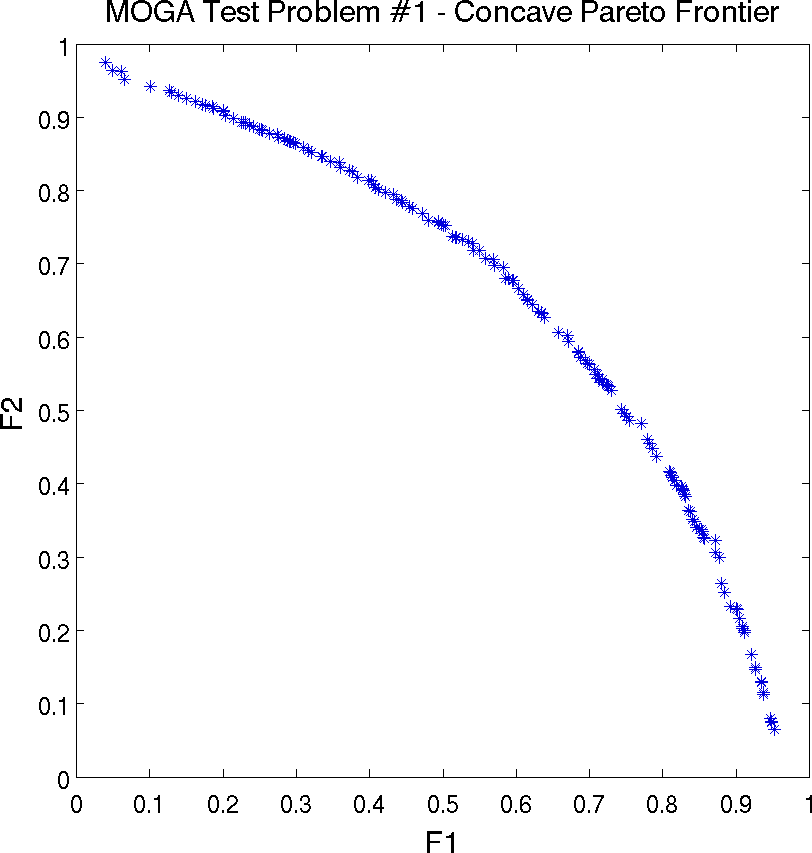
\includegraphics[scale=0.75]{images/dakota_mogatest1_pareto_front}
  \caption{Multiple objective genetic algorithm (MOGA) example: Pareto
  front showing tradeoffs between functions f1 and f2.}
  \label{tutorial:moga_pareto}
\end{figure}

Sections~\ref{opt:software} and~\ref{opt:additional} provide more
information on multiobjective optimization.  There are three detailed
examples provided in Section~\ref{additional:multiobjective}.

\subsection{Uncertainty Quantification}\label{tutorial:example:uncert_quant}

Uncertainty quantification (UQ) is the process of determining the
effect of input uncertainties on response metrics of interest.  These
input uncertainties may be characterized as either aleatory
uncertainties, which are irreducible variabilities inherent in nature,
or epistemic uncertainties, which are reducible uncertainties
resulting from a lack of knowledge.  Since sufficient data is
generally available for aleatory uncertainties, probabilistic methods
are commonly used for computing response distribution statistics based
on input probability distribution specifications.  Conversely, for
epistemic uncertainties, data is generally sparse, making the use of
probability theory questionable and leading to nonprobabilistic
methods based on interval specifications.

The subsection demonstrates the use of several methods of uncertainty 
quantification methods built into DAKOTA.  These examples include 
Monte Carlo random sampling, reliability methods, the representation 
of a stochastic process by a polynomial chaos expansion, 
and interval analysis.  

\subsubsection{Monte Carlo Sampling}\label{tutorial:example:uncert_quant:monte_carlo}

Figure~\ref{tutorial:rosenbrock_mc} shows the DAKOTA input file for
an example problem that demonstrates some of the random sampling
capabilities available in DAKOTA. In this example, the design
parameters, x1 and x2, will be treated as uncertain parameters that
have uniform distributions over the interval [-2, 2]. This is
specified in the variables section of the input file, beginning with
the keyword \texttt{uniform\_uncertain}.
% Not true: For comparison, the keywords
% from the previous examples are retained, but have been commented out.
Another change from earlier input files, such as
Figure~\ref{tutorial:rosenbrock_vector},
occurs in the responses section, where
the keyword \texttt{num\_response\_functions} is used in place of
\texttt{num\_objective\_functions}. The final changes to the input
file occur in the method section, where the keyword
\texttt{sampling} is used; ``nond'' is an abbreviation for 
nondeterministic.
The other keywords in the methods section of the input file
specify the number of samples (200), the seed for the random number
generator (17), the sampling method (random), and the response
threshold (100.0). The \texttt{seed} specification allows a user to
obtain repeatable results from multiple runs. If a seed value is not
specified, then DAKOTA's sampling methods are designed to generate
nonrepeatable behavior (by initializing the seed using a system
clock). The keyword \texttt{response\_thresholds} allows the user to
specify threshold values for which DAKOTA will compute statistics on
the response function output.  Note that a unique threshold value can
be specified for each response function.

In this example, DAKOTA will select 200 design points from within the
parameter space, evaluate the value of Rosenbrock's function at all
200 points, and then perform some basic statistical calculations on
the 200 response values.

This DAKOTA input file is executed using the following command:
\begin{small}
\begin{verbatim}
         dakota dakota_rosenbrock_nond.in > nond.out
\end{verbatim}
\end{small}

Figure~\ref{tutorial:results_mc} shows example results from this 
sampling method.  See the \texttt{nond.out.sav} file in directory
\texttt{Dakota/examples/tutorial} for comparison with results
produced by DAKOTA. Note that your results will differ from those in
this file if your \texttt{seed} value differs or if no \texttt{seed}
is specified.


As shown in Figure~\ref{tutorial:results_mc}, 
the statistical data on the 200 Monte Carlo samples is printed at the
end of the output file in the section that starts with ``Statistics
based on 200 samples.'' In this section, DAKOTA outputs the
mean, standard deviation, coefficient of variation, and 95\%
confidence intervals for each of the response functions.  For example, 
the mean of the Rosenbrock function given uniform input uncertainties 
on the input variables is 455.4 and the standard deviation is 536.8. 
This is a very large standard deviation, due to the fact that the 
Rosenbrock function varies by three orders of magnitude over the input 
domain.  The statistical information on moments in the output is followed by
the fractions (``Probability Level'') of the response function values 
that are below the response threshold values specified in the input file. 
For example, 34 percent of the sample inputs resulted in a Rosenbrock 
function value that was less than or equal to 100, as shown in the line 
listing the cumulative distribution function values.  
Finally, there are several 
correlation matrices printed at the end, showing simple and partial 
raw and rank correlation matrices.  Correlations provide an indication 
of the strength of a monotonic relationship between input and outputs.  
More detail on correlation coefficients and their interpretation can be 
found in Section~\ref{uq:uncertainty1}. 
More detail about sampling methods in general can be found in 
Section~\ref{uq:sampling}.  Finally,  
Figure~\ref{tutorial:rosenbrock_mc_points} shows the locations
of the 200 sample sites within the parameter space of the Rosenbrock
function for this example.

\begin{figure}[ht!]
  \centering
  \begin{bigbox}
    \begin{small}
      \verbatimtabinput[8]{dakota_rosenbrock_nond.in}
    \end{small}
  \end{bigbox}
  \caption{Monte Carlo sampling example: the DAKOTA input file.}
  \label{tutorial:rosenbrock_mc}
\end{figure}

\begin{figure}
\centering
\begin{bigbox}
\begin{footnotesize}
\begin{verbatim}
Statistics based on 200 samples:

Moment-based statistics for each response function:
                            Mean           Std Dev          Skewness          Kurtosis
 response_fn_1  4.5540183516e+02  5.3682678089e+02  1.6661798252e+00  2.7925726822e+00

95% confidence intervals for each response function:
                    LowerCI_Mean      UpperCI_Mean    LowerCI_StdDev    UpperCI_StdDev
 response_fn_1  3.8054757609e+02  5.3025609422e+02  4.8886795789e+02  5.9530059589e+02

Level mappings for each response function:
Cumulative Distribution Function (CDF) for response_fn_1:
     Response Level  Probability Level  Reliability Index  General Rel Index
     --------------  -----------------  -----------------  -----------------
   1.0000000000e+02   3.4000000000e-01

Simple Correlation Matrix among all inputs and outputs:
                       x1           x2 response_fn_1 
          x1  1.00000e+00 
          x2 -5.85097e-03  1.00000e+00 
response_fn_1 -9.57746e-02 -5.08193e-01  1.00000e+00 

Partial Correlation Matrix between input and output:
             response_fn_1 
          x1 -1.14659e-01 
          x2 -5.11111e-01 

Simple Rank Correlation Matrix among all inputs and outputs:
                       x1           x2 response_fn_1 
          x1  1.00000e+00 
          x2 -6.03315e-03  1.00000e+00 
response_fn_1 -1.15360e-01 -5.04661e-01  1.00000e+00 

Partial Rank Correlation Matrix between input and output:
             response_fn_1 
          x1 -1.37154e-01 
          x2 -5.08762e-01 
\end{verbatim}
\end{footnotesize}
\end{bigbox}
\caption{Results of Monte Carlo Sampling on the Rosenbrock Function}
\label{tutorial:results_mc}
\end{figure}


\begin{figure}[ht!]
  \centering
  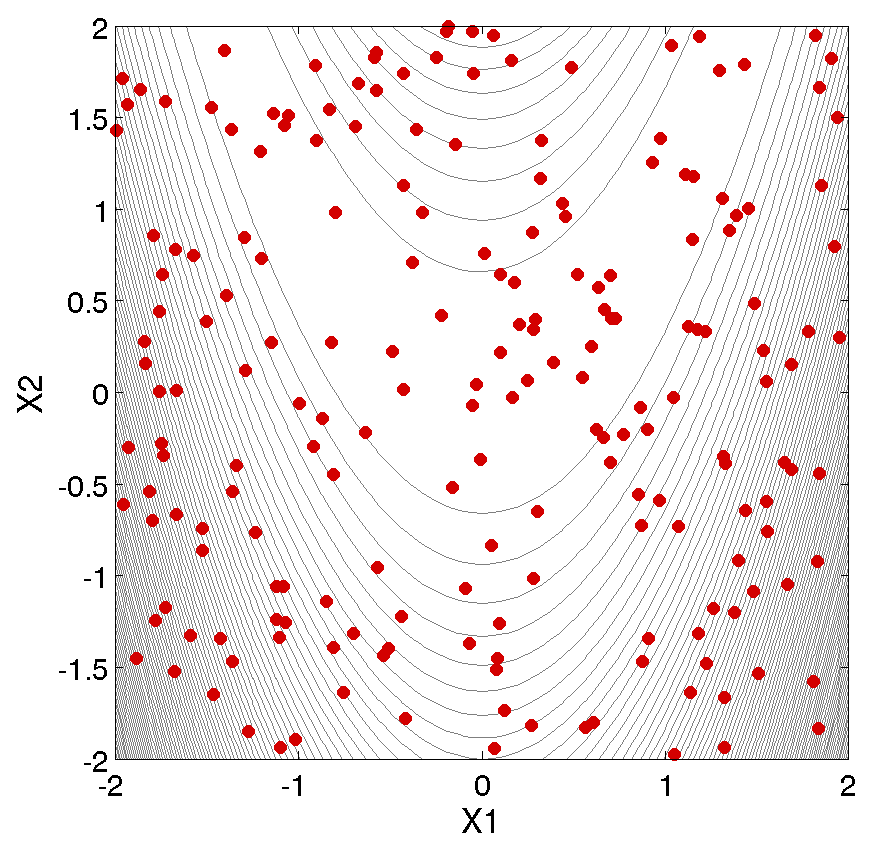
\includegraphics[height=2.5in]{images/rosen_nond_pts}
  \caption{Monte Carlo sampling example: locations in the parameter
    space of the 200 Monte Carlo samples using a uniform distribution
    for both $x_1$ and $x_2$.}
  \label{tutorial:rosenbrock_mc_points}
\end{figure}

%\newpage

\subsubsection{Reliability Methods - via the Mean Value Method}\label{tutorial:example:uncert_quant:reliability}

Reliability methods provide an alternative approach to uncertainty
quantification which can be less computationally demanding than
sampling techniques.  Reliability methods for uncertainty
quantification are based on probabilistic approaches that compute
approximate response function distribution statistics based on
specified uncertain variable distributions.  These response statistics
include response mean, response standard deviation, and cumulative or
complementary cumulative distribution functions (CDF/CCDF).  These
methods are often more efficient at computing statistics in the tails
of the response distributions (events with low probability) than
sampling based approaches since the number of samples required to
resolve a low probability can be prohibitive.

Figure~\ref{tutorial:textbook_mv} shows the DAKOTA input file for
an example problem that demonstrates the simplest reliability method, 
called the mean value method (also referred to as the Mean Value 
First Order Second Moment method).  It is specified with method 
keyword \texttt{local\_reliability}.  
This method calculates the mean 
and variance of the response function based on information about the 
mean and variance of the inputs and gradient information at the mean 
of the inputs. The mean value method is extremely cheap computationally 
(only five runs were required for the textbook function), but can 
be quite inaccurate, especially for nonlinear problems and/or problems 
with uncertain inputs that are significantly non-normal. More 
detail on the mean value method can be found in 
Section~\ref{uq:reliability:mv}, and more detail on reliability 
methods in general (including the more advanced methods) is found in 
Section~\ref{uq:reliability}.

Example output from the mean value method is displayed in 
Figure~\ref{tutorial:results_mv}. Note that since the mean of both inputs
is 1, the mean value of the output for response 1 is zero. 
However, the mean values of the constraints are both 0.5. 
The mean value results indicate that variable x1 is more 
important in constraint 1 while x2 is more important in constraint 2, 
which is the case based on Equation~\ref{tutorial:textbook_f}.

This DAKOTA input file is executed using the following command:
\begin{small}
\begin{verbatim}
         dakota dakota_mv.in > mv.out
\end{verbatim}
\end{small}
See the file \texttt{mv.out.sav} in \texttt{Dakota/examples/tutorial} 
for comparison with results from DAKOTA. 

\begin{figure}[ht!]
  \centering
  \begin{bigbox}
    \begin{small}
      \verbatimtabinput[8]{dakota_mv.in}
    \end{small}
  \end{bigbox}
  \caption{Mean Value Reliability Method: the DAKOTA input file.}
  \label{tutorial:textbook_mv}
\end{figure}

\begin{figure}
\centering
\begin{bigbox}
\begin{small}
\begin{verbatim}
-----------------------------------------------------------------
MV Statistics for response_fn_1:
  Approximate Mean Response                  =  0.0000000000e+00
  Approximate Standard Deviation of Response =  0.0000000000e+00
  Importance Factors not available.
MV Statistics for response_fn_2:
  Approximate Mean Response                  =  5.0000000000e-01
  Approximate Standard Deviation of Response =  1.0307764064e+00
  Importance Factor for variable TF1ln       =  9.4117647059e-01
  Importance Factor for variable TF2ln       =  5.8823529412e-02
MV Statistics for response_fn_3:
  Approximate Mean Response                  =  5.0000000000e-01
  Approximate Standard Deviation of Response =  1.0307764064e+00
  Importance Factor for variable TF1ln       =  5.8823529412e-02
  Importance Factor for variable TF2ln       =  9.4117647059e-01
-----------------------------------------------------------------
\end{verbatim}
\end{small}
\end{bigbox}
\caption{Results of the Mean Value Method on the Textbook Function}
\label{tutorial:results_mv}
\end{figure}


\subsubsection{Polynomial Chaos}\label{tutorial:example:uncert_quant:poly_chaos}
The term ``Polynomial Chaos'' refers to the representation of a stochastic 
process as a polynomial expansion in random (or stochastic) variables. This 
representation acts as a response surface that maps stochastic inputs to 
stochastic outputs.  Desired statistics can then be obtained from the 
response surface either analytically or by re-sampling the fast surrogate.
Exponential convergence of the error with increasing polynomial order can 
be obtained by using (an) orthogonal polynomial series whose weighting 
function(s) is/are the probability density functions of the stochastic 
inputs. Coefficients in the Chaos expansion are determined through
orthogonal projection. For non-intrusive implementations, such as in DAKOTA,
numerical integration via quadrature or cubature is used to evaluate the 
orthogonal projections.  Additional details regarding the method are 
provided in Section \ref{uq:expansion}.

A typical DAKOTA input file for performing an uncertainty
quantification using polynomial chaos expansions is shown in
Figure~\ref{tutorial:pce}.  In this example, we compute CDF
probabilities for six response levels of Rosenbrock's function.  Since
Rosenbrock is a fourth order polynomial and we employ a fourth-order
expansion using an optimal basis (Legendre for uniform random
variables), we can readily obtain a polynomial expansion which exactly
matches the Rosenbrock function.  In this example, we select Gaussian
quadratures using an anisotropic approach (fifth-order quadrature in
$x_1$ and third-order quadrature in $x_2$), resulting in a total of
15 function evaluations to compute the PCE coefficients.

\begin{figure}
  \centering
  \begin{bigbox}
    \begin{small}
      \verbatimtabinput[8]{dakota_pce.in}
    \end{small}
  \end{bigbox}
\caption{DAKOTA input file for performing UQ using polynomial chaos expansions.}
\label{tutorial:pce}
\end{figure}

The tensor product quadature points upon which the expansion is calculated 
are shown in Figure~\ref{tutorial:rosen_pce_points}.  
The tensor product generates
all combinations of values from each individual dimension: it is an 
all-way pairing of points.

\begin{figure}[ht!]
  \centering
  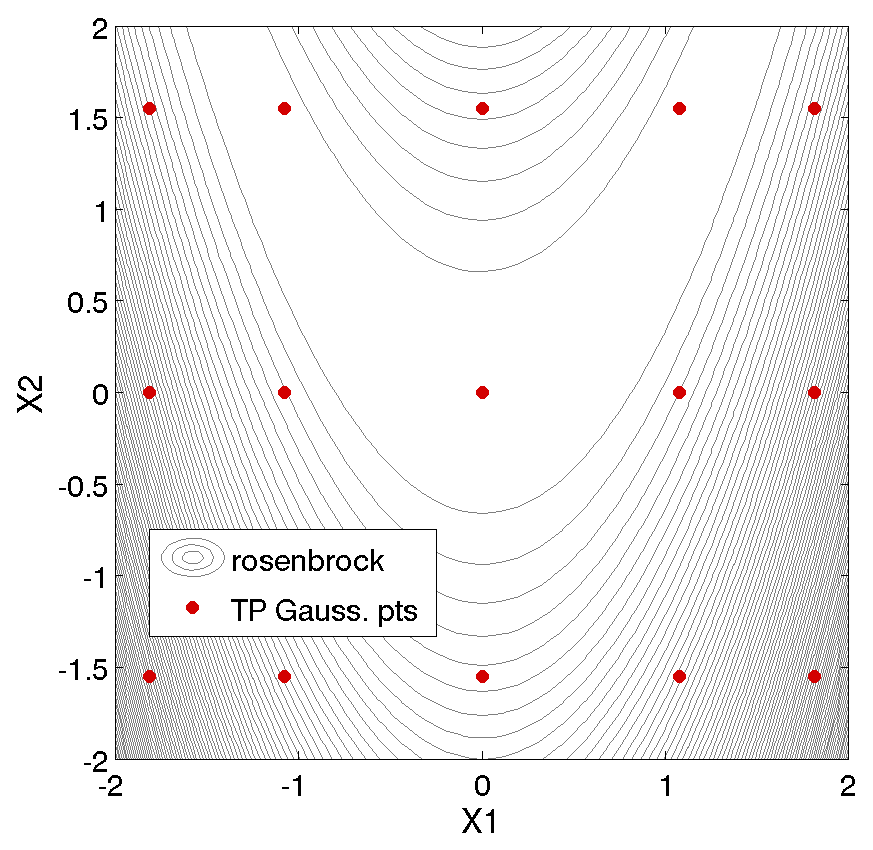
\includegraphics[height=2.5in]{images/rosen_pce_pts}
  \caption{Rosenbrock polynomial chaos example: tensor product quadrature points.}
  \label{tutorial:rosen_pce_points}
\end{figure}

Once the expansion coefficients have been calculated, some statistics
are available analytically and others must be evaluated numerically.
For the numerical portion, the input file specifies the use of 10000
samples, which will be evaluated on the expansion to compute the CDF
probabilities.  In Figure~\ref{tutorial:pce_out}, excerpts from the results
summary are presented, where we first see a summary of the PCE
coefficients which exactly reproduce Rosenbrock for a Legendre
polynomial basis.  The analytic statistics for mean, standard
deviation, and COV are then presented.  For example, the mean is 455.66 
and the standard deviation is 606.56.  The moments are followed 
by global sensitivity indices (Sobol indices).This example shows that variable 
x1 has the largest main effect (0.497) as compared with variable 
x2 (0.296) or the interaction between x1 and x2 (0.206). 
After the global sensitivity indices, the local, analytic random 
variable sensitivities are presented, evaluated at the mean values.
Finally, we see the numerical results for the CDF probabilities based
on 10000 samples performed on the expansion. For example, 
the probability that the Rosenbrock function is less than 100 
over these two uncertain variables is 0.342. Note that this is a very similar 
estimate to what was obtained using 200 Monte Carlo samples, with 
fewer function evaluations.
\begin{figure}
\centering
\begin{bigbox}
\begin{footnotesize}
\begin{verbatim}
Polynomial Chaos coefficients for response_fn_1:
        coefficient   u1   u2
        ----------- ---- ----
   4.5566666667e+02   P0   P0
  -4.0000000000e+00   P1   P0
   9.1695238095e+02   P2   P0
  -9.9475983006e-14   P3   P0
   3.6571428571e+02   P4   P0
  -5.3333333333e+02   P0   P1
  -3.9968028887e-14   P1   P1
  -1.0666666667e+03   P2   P1
  -3.3573144265e-13   P3   P1
   1.2829737273e-12   P4   P1
   2.6666666667e+02   P0   P2
   2.2648549702e-13   P1   P2
   4.8849813084e-13   P2   P2
   2.8754776338e-13   P3   P2
  -2.8477220582e-13   P4   P2
-------------------------------------------------------------------
Statistics derived analytically from polynomial expansion:

Moment-based statistics for each response function:
                            Mean           Std Dev          Skewness          Kurtosis
response_fn_1
  expansion:    4.5566666667e+02  6.0656024184e+02
  numerical:    4.5566666667e+02  6.0656024184e+02  1.9633285271e+00  3.3633861456e+00

Covariance among response functions:
[[  3.6791532698e+05 ]] 

Local sensitivities for each response function evaluated at uncertain variable means:
response_fn_1:
 [ -2.0000000000e+00  2.4055757386e-13 ] 

Global sensitivity indices for each response function:
response_fn_1 Sobol indices:
                                  Main             Total
                      4.9746891383e-01  7.0363551328e-01 x1
                      2.9636448672e-01  5.0253108617e-01 x2
                           Interaction
                      2.0616659946e-01 x1 x2 

Statistics based on 10000 samples performed on polynomial expansion:

Level mappings for each response function:
Cumulative Distribution Function (CDF) for response_fn_1:
     Response Level  Probability Level  Reliability Index  General Rel Index
     --------------  -----------------  -----------------  -----------------
   1.0000000000e-01   1.9000000000e-03
   1.0000000000e+00   1.3600000000e-02
   5.0000000000e+01   2.4390000000e-01
   1.0000000000e+02   3.4230000000e-01
   5.0000000000e+02   7.1090000000e-01
   1.0000000000e+03   8.5240000000e-01
-------------------------------------------------------------------
\end{verbatim}
\end{footnotesize}
\end{bigbox}
\caption{Excerpt of UQ output for polynomial chaos example.}
\label{tutorial:pce_out}
\end{figure}

\subsubsection{Interval Analysis}\label{tutorial:example:uncert_quant:interval}

Interval analysis is often used to model epistemic uncertainty. 
In interval analysis, one assumes that nothing is known about 
an epistemic uncertain variable except that its value lies 
somewhere within an interval.  In this situation, it is NOT 
assumed that the value has a uniform probability of occuring 
within the interval.  Instead, the interpretation is that 
any value within the interval is a possible value or a potential 
realization of that variable.  In interval analysis, the 
uncertainty quantification problem is one of determining the 
resulting bounds on the output (defining the output interval) 
given interval bounds on the inputs. Again, any output response 
that falls within the output interval is a possible output 
with no frequency information assigned to it.

We can do interval analysis using either
\texttt{global\_interval\_est} or \texttt{local\_interval\_est}.
In the global approach, one uses either a global optimization 
method or a sampling method to assess the bounds, whereas the 
local method uses gradient information in a derivative-based 
optimization approach. 
 
An example of interval estimation 
is found in the test file \texttt{dakota\_uq\_interval.in}, 
and also in Figure~\ref{tutorial:interval}, with example results in 
Figure~\ref{tutorial:interval_out}. This example is a demonstration 
of calculating interval bounds for three outputs of the cantilever beam 
problem. The cantilever beam problem is described in detail in 
Section~\ref{additional:cantilever}. Given input intervals of [1,10] on 
beam width and beam thickness, we can see that the interval estimate of 
beam weight is approximately [1,100].

\begin{figure}
  \centering
  \begin{bigbox}
    \begin{small}
      \verbatimtabinput[8]{dakota_uq_interval.in}
    \end{small}
  \end{bigbox}
\caption{DAKOTA input file for performing UQ using interval analysis.}
\label{tutorial:interval}
\end{figure}

\begin{figure}
\centering
\begin{bigbox}
\begin{small}
\begin{verbatim}
------------------------------------------------------------------
Min and Max estimated values for each response function:
weight:  Min = 1.0000169352e+00  Max = 9.9999830649e+01
stress:  Min = -9.7749994284e-01  Max = 2.1499428450e+01
displ:  Min = -9.9315677360e-01  Max = 6.7429714485e+01
-----------------------------------------------------------------
\end{verbatim}
\end{small}
\end{bigbox}
\caption{Excerpt of UQ output for interval example.}
\label{tutorial:interval_out}
\end{figure}

\subsection{User Supplied Simulation Code Examples}\label{tutorial:example:user_supply}
This subsection provides examples of how to use DAKOTA to drive user 
supplied black box code.

\subsubsection{Optimization with a User-Supplied Simulation Code - Case 1}\label{tutorial:example:user_supply:optimization1}

Many of the previous examples made use of the direct interface to
access the Rosenbrock and textbook test functions that are compiled
into DAKOTA. In engineering applications, it is much more common to
use the \texttt{system} or \texttt{fork} interface approaches within
DAKOTA to manage external simulation codes. In both of these cases,
the communication between DAKOTA and the external code is conducted
through the reading and writing of short text files. For this example,
the C++ program \texttt{rosenbrock.C} in \texttt{Dakota/test} is used
as the simulation code.  This file is compiled to create the
stand-alone \texttt{rosenbrock} executable that is referenced as the
\texttt{analysis\_driver} in Figure~\ref{tutorial:rosenbrock_user}.
This stand-alone program performs the same function evaluations as
DAKOTA's internal Rosenbrock test function.

Figure~\ref{tutorial:rosenbrock_user} shows the text of the DAKOTA
input file named \texttt{dakota\_rosenbrock\_syscall.in} that is
provided in the directory \texttt{Dakota/examples/tutorial}.
The only differences between this input file and the one in Figure~
\ref{tutorial:rosenbrock_grad} occur in the \emph{interface} keyword
section. The keyword \texttt{system} indicates that DAKOTA will use
system calls to create separate Unix processes for executions of the
user-supplied simulation code. The name of the simulation code, and
the names for DAKOTA's parameters and results file are specified using
the \texttt{analysis\_driver}, \texttt{parameters\_file}, and
\texttt{results\_file} keywords, respectively.

This example problem is executed using the command:
\begin{small}
\begin{verbatim}
    dakota dakota_rosenbrock_syscall.in > syscall.out
\end{verbatim}
\end{small}

This run of DAKOTA takes longer to complete than the previous
gradient-based optimization example since the \texttt{system}
interface method has additional process creation and file I/O
overhead, as compared to the internal communication that occurs when
the \texttt{direct} interface method is used. File
\texttt{syscall.out.sav} in the
\texttt{Dakota/examples/tutorial} directory permits comparison with
output results you get by executing the command given above.

To gain a better understanding of what exactly DAKOTA is doing with
the \texttt{system} interface approach, add the keywords
\texttt{file\_tag} and \texttt{file\_save} to the interface
specification and re-run DAKOTA. Check the listing of the local
directory and you will see many new files with names such as
\texttt{params.in.1}, \texttt{params.in.2}, etc., and
\texttt{results.out.1}, \texttt{results.out.2}, etc. There is one
\texttt{params.in.X} file and one \texttt{results.out.X} file for each
of the function evaluations performed by DAKOTA. This is the file
listing for \texttt{params.in.1}:
%\newpage
\begin{small}
\begin{verbatim}
                                          2 variables
                     -1.200000000000000e+00 x1
                      1.000000000000000e+00 x2
                                          1 functions
                                          1 ASV_1
                                          2 derivative_variables
                                          1 DVV_1
                                          2 DVV_2
                                          0 analysis_components
\end{verbatim}
\end{small}

\begin{figure}[b!]
  \begin{bigbox}
    \begin{small}
      \verbatimtabinput[8]{dakota_rosenbrock_syscall.in}
    \end{small}
  \end{bigbox}
  \caption{DAKOTA input file for gradient-based optimization using the
    system call interface to an external rosenbrock simulator.}
  \label{tutorial:rosenbrock_user}
\end{figure}

The basic pattern is that of array lengths and string identifiers
followed by listings of the array entries, where the arrays consist of
the variables, the active set vector (ASV), the derivative values
vector (DVV), and the analysis components (AC).  For the variables
array, the first line gives the total number of variables (2) and the
``variables'' string identifier, and the subsequent two lines provide
the array listing for the two variable values (-1.2 and 1.0) and
descriptor tags (``x1'' and ``x2'' from the DAKOTA input file).  The
next array conveys the ASV, which indicates what
simulator outputs are needed.  The first line of the array gives the total number
of response functions (1) and the ``functions'' string identifier,
followed by one ASV code and descriptor tag
(``ASV\_1'') for each function.  In this case, the ASV value of 1 indicates that DAKOTA
is requesting that the simulation code return the response function
value in the file \texttt{results.out.X}. (Possible ASV values: 1 = value of
response function value, 2 = response function gradient, 4 = response
function Hessian, and any sum of these for combinations up to
7 = response function value, gradient, and Hessian; see ~\ref{variables:asv} for
more detail.)  The next array provides the DVV, which defines the
variable identifiers used in computing derivatives.  The first line of
the array gives the number of derivative variables (2) and the
``derivative\_variables'' string identifier, followed by the listing of
the two DVV variable identifiers (the first and second variables) and
descriptor tags (``DVV\_1'' and ``DVV\_2'').  The final array provides
the AC array used to provide additional strings for use by the
simulator (e.g., to provide the name of a particular mesh file).  The
first line of the array gives the total number of analysis components
(0) and the ``analysis\_components'' string identifier, followed by the
listing of the array, which is empty in this case.

The executable program rosenbrock reads in the \texttt{params.in.X}
file and evaluates the objective function at the given values for
$x_1$ and $x_2$.  Then, rosenbrock writes out
the objective function data to the \texttt{results.out.X} file. Here
is the listing for the file \texttt{results.out.1}:
\begin{small}
\begin{verbatim}
                     2.420000000000000e+01 f
\end{verbatim}
\end{small}

The value shown above is the value of the objective function, and the
descriptor `f' is an optional tag returned by the simulation code.
When the system call has completed, DAKOTA reads in the data from the
\texttt{results.in.X} file and processes the results. DAKOTA then
continues with additional executions of the rosenbrock program until
the optimization process is complete.

\subsubsection{Optimization with a User-Supplied Simulation Code - Case 2}\label{tutorial:example:user_supply:optimization2}

In many situations the user-supplied simulation code cannot be
modified to read and write the \texttt{params.in.X file} and the
\texttt{results.out.X} file, as described above. Typically, this
occurs when the simulation code is a commercial or proprietary
software product that has specific input file and output file formats.
In such cases, it is common to replace the executable program name in
the DAKOTA input file with the name of a Unix shell script containing
a sequence of commands that read and write the necessary files and run
the simulation code. For example, the executable program named
\texttt{rosenbrock} listed in Figure~\ref{tutorial:rosenbrock_user}
could be replaced by a Unix C-shell script named
\texttt{simulator\_script}, with the script containing a sequence of
commands to perform the following steps: insert the data from the
\texttt{parameters.in.X} file into the input file of the simulation
code, execute the simulation code, post-process the files generated by
the simulation code to compute response data, and return the response
data to DAKOTA in the \texttt{results.out.X} file. The steps that are
typically used in constructing and using a Unix shell script are
described in Section~\ref{advint:building}.

\section{Where to Go from Here}\label{tutorial:where}

This chapter has provided an introduction to the basic capabilities of
DAKOTA including parameter studies, various types of optimization, and
uncertainty quantification sampling. More information on the DAKOTA
input file syntax is provided in the remaining chapters in this manual
and in the DAKOTA Reference Manual~\cite{RefMan}. Additional example
problems that demonstrate some of DAKOTA's advanced capabilities are
provided in Chapter~\ref{uq}, Chapter~\ref{sbm}, Chapter~\ref{strat},
Chapter~\ref{advint}, and Chapter~\ref{additional}.

Here are a few pointers to sections of this manual that many new users
find useful:

\begin{itemize}
\item Chapter~\ref{output} describes the different DAKOTA output file
  formats, including commonly encountered error messages.
\item Chapter~\ref{advint} demonstrates how to employ DAKOTA with a
  user-supplied simulation code.\\
  \emph{Most DAKOTA users will follow the approach described in Chapter~\ref{advint}.}
\item Chapter~\ref{usage} provides guidelines on how to choose an
  appropriate optimization, uncertainty quantification, or parameter
  study method based on the characteristics of your application.
\item Chapter~\ref{restart} describes the file restart and data re-use
  capabilities of DAKOTA.
\end{itemize}
